\documentclass[12pt,  a4paper, openright]{report} %twoside,
\usepackage{amsmath}
\usepackage[utf8]{inputenc}
\usepackage{graphicx}
\usepackage[hmargin=2cm,vmargin=2cm]{geometry}
\usepackage[francais]{babel}
\usepackage{color}
\usepackage{here}
\usepackage[Conny]{fncychap} % Sonny, Lenny, Glenn, Conny, Rejne, Bjarne
\usepackage{hyperref}
\usepackage{enumitem}
\usepackage{amssymb}
\usepackage{latexsym}


\def\lesssim{\mathrel{\hbox{\rlap{\hbox{\lower5pt\hbox{$\sim$}}}\hbox{$<$}}}}
\def\gtrsim{\mathrel{\hbox{\rlap{\hbox{\lower5pt\hbox{$\sim$}}}\hbox{$>$}}}}
\def\ni{\noindent}
\def\bfn{\mbox{\boldmath$\nabla$}}
\def\bfhl{\hat{{\mbox{\boldmath$\ell$}}}}



\definecolor{Zgris}{rgb}{0.87,0.85,0.85}
\newsavebox{\BBbox}
\newenvironment{DDbox}[1]{
	\begin{lrbox}{\BBbox}\begin{minipage}{\linewidth}}
		{\end{minipage}\end{lrbox}\noindent\colorbox{Zgris}{\usebox{\BBbox}} \\
	[.5cm]}




%\hypersetup{pdfborder={0 0 0},colorlinks,urlcolor=false,citecolor=blue,linkcolor=blue}
\renewcommand\thefootnote{\textcolor{blue}{\arabic{footnote}}}
\newcommand{\reporttitle}{Physique des trous noirs: thermodynamique et transitions de phase}     % Titre
\newcommand{\reportauthor}{Ismail  \textsc{EZZAKI}} % Auteur
\newcommand{\reportsubject}{\textbf{Mémoire}\\présenté pour obtenir le diplôme de master en: \\
	\textbf{Physique des Hautes Énergies, Astrophysique et Physique computationnelle  }  } % Sujet
\newcommand{\HRule}{\rule{\linewidth}{0.7mm}}


\newcommand{\chaptertoc}[1]{\chapter*{#1}
	\addcontentsline{toc}{chapter}{#1}
	\markboth{\slshape\MakeUppercase{#1}}{\slshape\MakeUppercase{#1}}}


\newcommand{\be}{\begin{equation}}
\newcommand{\ee}{\end{equation}}
\newcommand{\ba}{\begin{eqnarray}}
\newcommand{\ea}{\end{eqnarray}}


\begin{document}

\begin{titlepage}
	
	\begin{figure}[h!]
		\begin{minipage}[b]{0.25\linewidth}
			\begin{center}
		%		\includegraphics[width=20mm]{images/un.png}
			\end{center}
			
		\end{minipage}\hfill
		\begin{minipage}[b]{0.45\linewidth}   
			\begin{center}
		%		\includegraphics[width=40mm]{images/sem.png}
			\end{center}
			
		\end{minipage}
		\begin{minipage}[b]{0.27\linewidth}
			\begin{center}
		%		\includegraphics[width=33mm]{images/labo.png}
			\end{center}
			
		\end{minipage}\hfill
		
	\end{figure}
	\begin{center}
		\huge{ Université Cadi Ayyad} \\
		\large Faculté des Sciences Semlalia\\
		Laboratoire de Physique des Hautes Énergies et Astrophysique
	\end{center}
	
	\HRule 
	\begin{center}
		
		{\Large \reportsubject}\\[0.5cm]
		\vspace{0.4cm}
		
		
		\Large Sous le thème:\\
		\HRule \\[0.8cm]
		{\Huge \bfseries \reporttitle}\\[0.4cm]
		
		\HRule \\[0.8cm]
		
		\begin{Large}
			
			\begin{minipage}[b]{0.45\linewidth}
				\begin{flushleft}
					\emph{Auteur :}\\
					\reportauthor
				\end{flushleft}       
			\end{minipage}
			\begin{minipage}[b]{0.45\linewidth}   
				\begin{flushright}
					\begin{tabular}{l}
						Sous la direction de: \\
						Mohamed \textsc{CHABAB} 
		
					\end{tabular}
					
				\end{flushright}   
			\end{minipage}\hfill
			
			
			
		\end{Large}
		
		
		%\vfill
		\vspace{0.5cm}
		%{\large }
		
	\end{center}
	\begin{flushleft}
		Soutenu le 19  Juillet 2019 devant la commission d'examen:\\ \vspace{1cm}
		
		\begin{minipage}{0.45\linewidth}
			\begin{itemize}
				\item[-] Prof:  \textsc{A.Adhchour}
				\item[-] Prof:  \textsc{M.Oulne}
				\item[-] Professeur:  \textsc{M.Chabab}
				
			\end{itemize}
		\end{minipage}\hfill
		\begin{minipage}{0.55\linewidth}
			\begin{itemize}
				\item[-] P.E.S Université Cadi Ayyad de Marrakech
				\item[-] P.E.S Université Cadi Ayyad de Marrakech
				\item[-] P.E.S Université Cadi Ayyad de Marrakech
				
			\end{itemize} 	     
		\end{minipage}
		
		
	\end{flushleft}
	\vspace{0.8cm}
	\begin{center}
		Année universitaire 2018/2019
	\end{center}
\end{titlepage}


\newpage
 
\begin{center}
\begin{LARGE}
	\textit{Remerciement\vspace*{2cm}}\\
\end{LARGE}

\end{center}

\textit{ Au terme de la rédaction de ce mémoire,je tiens tout d'abord à remercie sincèrement Mr \textbf{Mohamed Chabab} ,professeur au département de Physique de la Faculté des Sciences Semlalia et directeur du laboratoire de physique des hautes énergies etastrophysique,pour son suivi et pour son énorme soutien,qu'il n'a cessé de nous prodiguer tout au long de la période du projet .\\
	\\
	\\
	J'adresse toute ma gratitude à Monsieur Le Professeur\textbf{Mustapha Oulne}  et à Monsieur Le
	Professeur \textbf{Abdrahim Adahchour}  d'avoir immédiatement accepté d'être membres de ce jury.\\
	\\
	\\
%	Je tiens à remercier particulièrement Monsieur \textbf{Samir IRAOUI}, doctorant de LPHEA, qui
%	n'a pas été avare de son temps, il m'a beaucoup aidé tout au long de cette expérience, et m'a
%	fourni les outils nécessaires pour faire ce travail.\\
%	\\
%	\\
	Je tiens à remercier aussi toute l’équipe pédagogique de la faculté des Sciences Semlalia pour
	les efforts fournis pour préparer les conditions de travail optimales.\\
	\\
	\\
	Je suis particulièrement sensible à la très bonne ambiance du Laboratoire de Physique des Hautes
	Énergies et Astrophysique .\\
	\\
	\\
	Enfin,je dédie ce modeste travail à mes parents,mes frères , mes amis et Ceux qui ont partagé avec moi tous les moments d'émotion lors de la réalisations de ce travail.}



\tableofcontents


\input{chapter/introduction}
	\chapter{Les trous noirs en astrophysique}
L’astrophysique est une science dont l’objet est l’étude physique des corps célestes. Elle
se propose d’interpréter et d’unifier les données observées par la recherche astronomique
en élaborant des lois physiques qui peuvent les expliquer \cite{2}. On s’intéresse dans ce
chapitre d’étudier les trous noirs en Astrophysique.
	\section{Formation des trous noirs}
	
	Les étoiles, à la fin de leur vie, connaissent des destins très différents dont la nature
dépend de la masse initiale de l’étoile. En effet, les réactions de fusion nucléaire qui ont lieu
dans les noyaux des étoiles produisent des éléments de plus en plus lourds en commençant
par l’hydrogène.
Une étoile peu massive comme le soleil, ne peut pas aller très loin dans la fusion,
son noyau se contracte pour devenir une naine blanche de masse inférieure à environ 1,4
masses solaires (limite de Chandrasekhar).


Quand aux étoiles plus massives, qui explosent sous forme de supernova du type II 1 .
Les parties extérieures de l’étoile se dispersent dans l’espace, alors que son noyau s’effondre
complètement sous son propre poids. Si après la supernova de type II, le noyau restant
est très massif $M bigger than M_Soleil$ , aucune force répulsive connue à l’intérieur d’une étoile ne
peut repousser assez fort pour empêcher l’étoile à s’effondrer sur lui-même en quelques
secondes. La matière se comprime rapidement, et cette matière dense forme le trou noir,

Quand le trou noir est formé, il faudrait une vitesse supérieure à la vitesse de la lumière
pour s’échapper de son champ gravitationnel, qui est très intense. Aucun objet ne peut
atteindre une vitesse plus grande que celle de la lumière, alors aucune matière ou radiation
ne peut s’échapper.

N’importe quel objet ayant une masse M suffisamment comprimée, peut devenir un
trou noir. Il suffit d’avoir un rayon égale au rayon de Schwarzschild correspondant.

	
	
	
	
	
	
	
	
	
	Pour la plupart des personnes qui savent ce qu’est un trou noir, il pense que l’origine d’un trou noir est absolument la mort d’une étoile or tous les astres de l’univers peuvent former un trou noir, en effet, pour former un trou noir il faut une masse élevée .Prenons tout d’abord une étoile de taille moyenne c'est-à-dire dont la masse est à peu près égale à la masse du Soleil (de 0.5 à 4 masses du Soleil). Une fois que l’étoile à utiliser tout son réservoir en hydrogène l’étoile entame son réservoir en hélium mais le rythme de la fusion nucléaire de l’hélium pour donner du carbone s’accélère pour donner une étoile appelée Géante rouge.  Ensuite la vie de l’étoile n’est pas encore complètement finie en effet après avoir utiliser toutes ces réserves en hélium pour former du carbone et de l’oxygène. A ce stade les étoiles sont alors dépourvu de toutes les couches de gaz autour d’elle alors le noyau de celle-ci commence alors à se refroidir pour obtenir une faible température , cette étoile devient alors une Naines Blanches.\\ 
	Si on prend une étoile de masse comprise entre quatre et dix masses du Soleil environ alors on obtient une Super Géante rouge qui ont les mêmes propriétés que les Géantes Rouges mais avec une masse supérieure à dix masses solaires. Quand les Super Géantes commencent à ne plus avoir assez de combustibles pour faire des réactions de fusion thermodynamique, celles-ci commencent alors à s’effondrer sur elles mêmes et à cause de leur très grande masse ces étoiles parviennent alors à former de très grandes réactions qui par leur force forment alors des supernovas, les restes de la Super Géantes alors se trouvent dans l’univers comme ceux-ci sont très proches et de très faibles tailles, puisque ce sont des protons et des électrons, il se recombinent pour former des neutrons et ainsi continuer à « vivre » pour former une étoile à neutrons de très faibles diamètres (environ 20 km) elles sont aussi appelées pulsars.\\
	Maintenant prenons une étoile dont la masse est supérieure à dix masses solaires alors quand l’étoile commence à ne plus avoir assez de carburant (hélium et hydrogène) celle-ci s’effondre mais ne laisse pas place à une supernova et une étoile à neutron comme les Super Géantes en effet celle-ci s’effondre mais comme leur gravité est très importante puisque leur masse est aussi très grande alors elle s’effondre et comme elle n’a plus de carburant elle ne peut plus effectuer une réaction chimiques pour s’enlever de sa force de gravité et de plus sa taille diminue aussi à grande vitesse jusqu’à atteindre la limite de d’Oppenheimer- Volkoff.\\
	À partir de cette limite l’effondrement est tel que plus aucune particule ou autre rayon comme la lumière ne peut s’en échapper et on assiste alors à la formation d’un trou noir.\\
	En astrophysique, la limite d'Oppenheimer-Volkoff, du nom de deux physiciens qui la calculèrent la première fois, représente la masse maximale théorique que peut avoir une étoile à neutrons. Au-delà de cette valeur, l'objet s'effondre alors en trou noir. La valeur de cette limite est d'environ 3,3 masses solaires et est à comparer avec la limite de Chandrasekhar pour les naines blanches. Cette limite est la valeur de la masse maximum du coeur de l'étoile \cite{3}.
	\begin{center}
		
	\end{center}
	Figure 1.1 –Les étapes de formation d’un trou noir
	\section{Les différents types de trous noirs}
	En fonction de leur masse, on distingue quatre types de trous noirs.
	\subsection{ trous noirs stellaires }
	La grande majorité des trous noirs seraient d’origine stellaire, c'est-à-dire de l’effondrement gravitationnel d’une vieille étoile massive sur elle-même. Ceux-ci ont une masse d'au moins quelques masses solaires. Ce type de trou noir ne fait que quelques kilomètres de diamètre. Leur formation peut engendrer des ondes gravitationnelles.
	Les principaux progéniteurs de trous noirs stellaires par effondrement sont les étoiles Wolf-Rayet qui est une étoile chaude, massive et évoluée présentant un taux de perte de masse très élevé . 
	\subsection{ Les trous noirs supermassifs }
	La formation des trous noirs supermassifs est encore fortement débattue car elle se fait sur de grandes échelles de temps (contrairement à la formation d’un trou noir stellaire). Comme il n’existe pas d’étoile de masse si grande, les trous noirs supermassifs ne peuvent pas directement être conçut d’un effondrement stellaire.Il pourrait s’agir d’une étoile massive qui s’effondre et qui donne naissance à un trou qui grandit peu à peu en se nourrissant d’autres étoiles ou bien d’un énorme nuage de gaz qui s’écroule directement sous sa propre gravité. Bien que l’origine des trous noirs supermassifs ne soit pas clairement définie, leur existence est en tout cas tout à fait possible.\\ 
	En astrophysique, un trou noir supermassif est un trou noir dont la masse est d’environ un million à un milliard de masse solaires .La densité de ce genre de trou noir  est très faible (parfois plus faible que celle de l’eau), des études montrent que plus un trou noir est grand, plus sa densité diminue, même si sa masse croit sans limite.
	\begin{figure}[H]
			\begin{center}
		
	\end{center}

	 \caption{Le trou noir supermassif est situé au centre de la galaxie .}
	
	\end{figure}
	\subsection{ Les trous noirs intermédiares }
	Les trous noirs intermédiaires sont des objets récemment découverts, de masse entre 100 et
	10 000 masses solaires. On peut donc dire que les trous noirs intermédiaires ne peuvent pas se former par simple effondrement d’étoiles massives.\\
	En Novembre 2004,une équipe d’astronome découvre le premier trou noir intermédiaire, orbitant à 3 années-lumières seulement au centre de notre galaxie. C’est un trou noir de 1 300 masses solaires. Grâce à ces observations, nous pouvons dire que les trous noirs de masse intermédiaire jouent un rôle dans la formation des trous noirs supermassifs.
	\subsection{ Les trous noirs primordiaux } 
	Ce type de trou noir ne peut pas être expliqué de la même manière que les trois précédents puisque celui-ci n'a jamais été vraiment prouvé, ce n'est que une hypothèse.\\ 
	Leur existence, toujours hypothétique, remonterait au début de la création de notre univers, il y a de cela 13,7 milliards d'années, bien avant l’émission de la première lumière de l'Univers.Son Masses Solaires n'ont pas été totalement définies, elles sont juste bien plus faible que celle des autres trous noirs.\\
Contrairement aux autres trous noirs, les trous noirs primordiaux perdent leur masse
de plus en plus rapidement et finissent par disparaître. Ce phénomène a été baptisé "évaporation quantique " par Stephen Hawking en 1975 \cite{4}.
	\section{Détection des trous noirs } 
	Les trous noirs, par leur caractère « invisible » ne se détectent que par leurs effets sur l’environnement. On peut distinguer deux grandes catégories de méthodes de détection :
	- quand le trou noir est accompagné d’une étoile « normale », on parle alors	
	de système binaire.
	- quand le trou noir est seul, on le dit alors célibataire.	
	\subsection{ Trou noir dans un système binaire }
	Etant donné son fort champ gravitationnel, le trou noir peut avoir une étoile comme satellite. C’est l’étude de la lumière émise par cette dernière qui nous permet de détecter le trou noir : dans un système binaire, les deux astres tournent l’un autour de l’autre. Lorsqu’on mesure le spectre infrarouge de l’étoile, on s’aperçoit qu’il varie périodiquement. Ceci est une application de l’effet redshift.
	Ce spectre prouve que l’étoile tourne autour d’un objet massif et invisible qui peut être soit une naine blanche, soit une étoile à neutrons, soit un trou noir. Pour faire la distinction, on mesure la masse de l’astre invisible en analysant son spectre, comme les étoiles à neutrons et les naines blanches ont une masse limite, si cette dernière est dépassée, le compagnon invisible est un trou noir.\\
	\begin{figure}[H]
		\begin{center}
			\centering

\caption{Conséquences de la variation de la longueur d'onde sur le spectre d'une étoile .}

	\end{center}
\end{figure}

	
	Il existe un autre moyen de détecter les trous noirs dans des systèmes binaires. En effet, lorsqu’une étoile est proche d’un trou noir, elle lui cède de sa matière. Cette matière est inexorablement attirée par le trou noir et tourne autour de celui-ci en formant un disque d'accrétion. En se rapprochant de la singularité, la matière s’échauffe et émet des rayons X. Cette émission est aléatoire car le disque d’accrétion, par son extrême chaleur, est très instable ; il se produit alors des « bulles chaudes » provoquant des sursauts de rayons X \cite{5}.
	Pour différencier l’étoile à neutrons du trou noir, on doit observer le centre du disque d’accrétion :\\
	- celui d’une étoile à neutrons est lumineux en raison de la matière	
	qui heurte la surface de l’étoile effondrée.\\
	- par contre, celui d’un trou noir sera sombre car la matière aura été	
	aspirée et donc aucune lumière ne nous arrivera.
	\begin{figure}[H]
		
	
	\begin{center}
		
	\end{center}
	\caption{Différence entre un trou noir et un étoile à neutrons.} 
\end{figure}
	
	\subsection{ Trou noir célibataire }
	Un trou noir célibataire est difficile à détecter ; le meilleur moyen est d’utiliser ses propriétés liées à la lumière, et notamment l'effet de lentille gravitationnelle.
	
	Les trous noirs dévient la trajectoire des rayons lumineux , c'est pourquoi on peut avoir deux images identiques d'une même étoile située derrière le trou noir.\\
	\begin{figure}[H]
	\begin{center}
		\centering
			
	\end{center}
\caption{l'effet lentille gravitationnelle.}
\end{figure}
	
	Dans la réalité, les deux images de l’étoile sont très proches voir confondues ce qui donne une étoile très lumineuse qui, si elle est détectée, nous informera sur la présence d’un corps céleste qui peut s’avérer être un trou noir.
	Comme pour les trous noirs dans les systèmes binaires, on peut les détecter grâce à leur rayonnement X. En effet, le trou noir célibataire possède lui aussi un disque d’accrétion : la méthode utilisée pour la détection d’un trou noir en système binaire peut donc être appliquée. Cependant, le disque d’accrétion d’un trou noir célibataire est très faible et devient indétectable par nos instruments de mesures s'ils sont distants de plus de 10 années-lumière.
	La détection d’un trou noir célibataire reste donc très théorique, même si on a réussi à observer un exemple flagrant de lentille convergente gravitationnelle.
	
	\section{Propriétés des trous noirs }
	Quasi toutes les propriétés des objets tombés dans le trou noir disparaissent. Seules subsistent trois propriétés : la masse, la charge électrique et le moment angulaire. C’est le théorème de la calvitie démontré par Werner Israel en 1967 : un trou noir (on dit qu'il n'a pas de poils) est entièrement connu par ces trois caractéristiques.\\
	On a dès lors quatre trous noirs possibles : celui qui a une masse sans charge électrique et qui ne tourne pas sur lui-même (trou noir de Schwarszchild), celui qui a une masse plus une charge électrique et qui ne tourne pas sur lui-même  (trou noir de Reissner-Nordström) et celui qui a une masse sans charge et un moment cinétique ( trou noir de Kerr),et enfin celui qui a une masse ,une charge et un moment cinétique (trou Kerr Neumann) quatre solutions exactes des équations de la relativité (voir le chapitre 2). 
		
		\begin{table}[H]
			\begin{center}
			\centering
		
			{ \renewcommand{\arraystretch}{1.9}
				
				\begin{tabular}{|l|l|l|}
					\hline
					& $J=0$ & $J\neq 0$\\
					\hline
					$Q=0$ & Schwarzschild &  Kerr \\
					
					\hline
					$Q\neq 0$ & Reissner-Nordstrom  & Kerr-Neweman \\
					\hline
					
					\hline
					
			\end{tabular}}
			\end{center}
			\caption{Les types théoriques du trou noir.}
		\end{table}
		
	
	\newpage 	

	\chapter{Les trous noirs en relativité générale}

 \section{Introducion}
 TODO
 
 La relativité générale est une théorie de la gravité. Elle se compose de deux parties. D'une part, il y a une description de la courbure de l'espace-temps, qui décrit le comportement des particules. D'autre part, il y a les équations du champ d'Einstein, qui décrivent comment l'énergie-momentum courbe l'espace-temps. 
 
 La relativité générale est construit sur la théorie spéciale de la relativité, qui est incluse dans le principe d'équivalence:
  «Dans un champ de gravitation, il est toujours possible, en tout point de l’espace, de choisir un référentiel (inertiel) dans lequel les lois de la physique sont localement identiques à celles en l’absence du champ de gravitation».

  Notez qu'en GR, il n'est pas possible d'étendre nos coordonnées à l'ensemble de
l'espace-temps. Dans un système de coordonnées locales, la gravité n'est pas perceptible et s'il y a
aucune autre force, l'objet se déplace en ligne droite et on a : 
	\begin{equation}
	\frac {d^{2}\xi^\alpha} {d\tau^{2} }= 0
	\end{equation}
	
 Dans un autre système de coordonnées $ x^\mu = x^\mu(\xi^\alpha)$ cette equation devient :

 $${d^2 x^\lambda \over d\tau^2} + \Gamma^\lambda_{\mu\nu}{dx^\mu \over
d\tau}  {dx^\nu \over d\tau}= 0, \eqno(3)$$
 

Cette équation de mouvement est connue sous le nom d'équation géodésique, où la connexion affine est définie comme

$$\Gamma^\lambda_{\mu\nu} = {\partial x^\lambda \over \partial
\xi^\alpha} \ \ {\partial^2 \xi^\alpha \over \partial x^{\mu}dx^\nu}
\eqno (4)$$

le temps propre est défini par:
$$d\tau^2 := \eta_{\mu\nu} d\xi^\mu d\xi^{\nu},$$
$$(\eta_{\mu\nu} = +1,\ -1,\ -1,\ -1 ).$$

Il peut également être écrit en coordonnées générales:
$$d\tau^2 := g_{\mu\nu} dx^\mu dx^{\nu},$$

où le tenseur métrique $g_{\mu\nu}$

 $$g_{\mu\nu} = {\partial \xi^\alpha \over \partial x^\mu}  {\partial \xi^\beta
\over \partial x^{\nu}} \eta_{\alpha\beta},$$

Les symboles ChristoUel $\Gamma^\sigma_{\mu\lambda} $ sont


$$\Gamma^\sigma_{\mu\lambda} = {1 \over 2}g^{\sigma\nu} 
\left [ {\partial g_{\mu\nu} \over \partial x^\lambda} +
{\partial g_{\lambda\nu} \over \partial x^\mu} -
{\partial g_{\mu\lambda} \over \partial x^\nu} \right ] . \eqno(7)$$

	\section{ Les équations d’Einstein}
	L’équation d'Einstein ou équation du champ d'Einstein, publiée par Albert Einstein, pour la première fois le 25 novembre 1915, est l'équation aux dérivées partielles principales de la relativité générale. C'est une équation dynamique qui décrit comment la matière et l'énergie modifient la géométrie de l'espace-temps. Cette courbure de la géométrie autour d'une source de matière est alors interprétée comme le champ gravitationnel de cette source. Le mouvement des objets dans ce champ est décrit très précisément par l'équation de sa géodésique.
	
	On ne peut pas démontrer les équations d’Einstein. Toutefois on peut argumenter de la
	façon suivante :\\
	$\ast$ C’est l’équation la plus simple possible satisfaisant au principe précédent.\\
	$\ast$ Elle est mathématiquement cohérent et définit un problème de valeurs initiales.\\
	$\ast$ Elle redonne l’équation de Newton dans une limite appropriée (la limite non relativiste).\\
	\\
	
	TODO
	\begin{equation}
 	T^{\alpha \beta} (x)= \sum_n{\frac{p^{\alpha}_n p^{\beta}_n} {p^{0}_n} \delta^{3} (x-x_n(t)) }
 	\end{equation}
	
	
	La forme mathématique de l’équation d’Einstein s’écrit \cite{7}
	\begin{equation}
	R_{\mu\nu}-\dfrac{1}{2}Rg_{\mu\nu}+g_{\mu\nu}\Lambda=8\pi GT_{\mu\nu}
	\end{equation}
	
	-$ R_{\mu\nu}$ : est le tenseur de Ricci, calculé à partir de la courbure de Riemann : $R_{\alpha\beta}$ =$ R_{\mu\alpha\mu\beta}$\\
	\\
	-$g_{\mu\nu}$ est la métrique de l’espace temps.\\
	\\
	-R : scalaire de Ricci.\\
	\\
	- $\Lambda$: constante cosmologique.\\
	\\
	- G : constante gravitationnelle de Newton.\\
	\\
	-$T_{\mu\nu}$: est le tenseur d’énergie-impulsion.\\
	\\
	où la courbure de Riemann et le symbole de Christoffel :
	\begin{equation}
	R_{\beta\gamma\delta}^{\alpha}= \partial_{\gamma}\Gamma_{\beta\delta}^{\alpha}-\partial_{\delta}\Gamma_{\beta\delta}^{\varepsilon}+ \Gamma_{\beta\delta}^{\varepsilon}         \Gamma_{\varepsilon\gamma}^\alpha- \Gamma\Gamma_{\beta\gamma}^{\varepsilon}\Gamma_{\varepsilon\delta}^{\alpha}
	\end{equation}
	
	
	\begin{equation}
	\Gamma_{\alpha\beta\gamma} = \dfrac{1}{2}( \partial_{\alpha}g_{\beta\gamma}+\partial_{\delta}g_{\gamma\alpha}-\partial_{\gamma}g_{\alpha\beta})
	\end{equation}
	
	Il est possible d’obtenir l’équation d’Einstein à partir du principe de moindre action, avec
	l’action d’Einstein-Hilbert définie par $(\Lambda = 0)$ :
	\begin{equation}
	S_{EH} = \int (L_{G} + L_{M})\sqrt{-g} d^{4}x =  \int\left(\dfrac{R}{2k} + L_{M} \right)\sqrt{-g} d^{4}x
	\end{equation}
	avec $L_{G}$ et $L_{M}$ représentent la densité lagrangienne de la gravité et de la matière présente
	respectivement, où $k = \dfrac{8Gpi}{c^{4}}$  et$ \sqrt{-g} = d^{4}x$ est l’élément de volume spatio-temporel peu importe le système de référence.\\
	Le principe de moindre action stipule qu’une variation de l’action d’Einstein-Hilbert par rapport
	à la métrique inverse doit être nulle ce qui nous permet d’obtenir :
	\begin{equation}
	\dfrac{\delta S_{EH}}{\delta g^{\mu\nu}} = \int\left[\dfrac{1}{2k}\dfrac{\delta (\sqrt{-g}R)}{
		\delta g^{\mu\nu}}+\dfrac{\delta \sqrt{-g}L_{M}}{\delta g^{\mu\nu}} \right]\delta g^{\mu\nu}d^{4}x
	\end{equation}
	\begin{equation}
	= \int\left[\dfrac{1}{2k}\dfrac{\delta R}{\delta g^{\mu\nu}}+\dfrac{1}{2k}\dfrac{R\delta \sqrt{-g}}{\sqrt{-\sqrt{g}\delta g^{\mu\nu}}}+\dfrac{1}{\sqrt{-g}}\dfrac{\delta L_{M}}{\delta g^{\mu\nu}}\right]\delta g^{\mu\nu}\sqrt{-g}d^{4}x 
	\end{equation}
	
	$$=0$$
	Danc on trouve:
	\begin{equation}
	\dfrac{\delta R}{\delta g^{\mu\nu}}+\dfrac{R\delta\sqrt{-g}}{\sqrt{-g}\delta g^{\mu\nu}}=-2k\dfrac{1}{\sqrt{-g}}\dfrac{\delta L_{M} }{\delta g^{\mu\nu}}
	\end{equation}
	
	alors:
	$$\dfrac{\delta R}{\delta g^{\mu\nu}}=R_{\mu\nu}$$ et $$\dfrac{R\delta\sqrt{-g}}{\sqrt{-g}\delta g^{\mu\nu}}=-\dfrac{1}{2}Rg_{\mu\nu}$$
	et on définisse le tenseur d'énergie à partir de $L_{M}$  $$T_{\mu\nu}=-2k\dfrac{1}{\sqrt{-g}}\dfrac{\delta L_{M} }{\delta g^{\mu\nu}}$$
	
	Danc La forme mathématique de l’équation d’Einstein s’écrit  :
	\begin{equation}
	R_{\mu\nu}-\dfrac{1}{2}Rg_{\mu\nu}=T_{\mu\nu}
	\end{equation}
	
	\section{The Newtonian limit}
	
Lets start with the equation of motion 
$$
{d^2x^\mu \over d\tau^2}  +\Gamma^\mu_{\lambda\nu}
{dx^2 \over d\tau}
{dx^\lambda \over d\tau}
= 0. \eqno (12)
$$
and let us assume  that the particles moves slowly
$${d{\bf x} \over d\tau} \ll 
{dt \over d\tau}, \ \ 
v\ll c.$$
If the particle moves slowly, {\it we can ignore the three-velocity terms}
in (12),
$${d^2x^\mu \over d\tau^2} + 
\Gamma^\mu_{00}\; c^2
\left ({dt \over d\tau}\right )^2 =0 .\eqno (13)
$$
Assume further that the gravitational field is stationary, then all
time derivatives of $g_{\mu\nu}$ are zero.  

Recall the equation relating the affine connection to the metric tensor,
\begin{eqnarray*}
\Gamma^\mu_{\lambda\nu} & = &
{1\over 2} g^{\kappa\mu} \left \{
{\partial g_{\nu\kappa}\over \partial x^\lambda} + 
{\partial g_{\lambda\kappa} \over \partial x^\nu} -
{\partial g_{\nu\lambda} \over \partial x^\kappa}
\right \} .
\end{eqnarray*}
Then the components appearing in equation (13) are
\begin{eqnarray*}
\Gamma^\mu_{00} & = & 
{1\over 2}g^{\kappa\mu} \left \{
{\partial g_{0\kappa} \over \partial x^0} +
{\partial g_{0\kappa} \over \partial x^0} -
{\partial g_{00} \over \partial x^\kappa}
\right \}\\
& = & 
- {1\over 2}g^{\kappa\mu} 
{\partial g_{00}\over \partial x^\kappa}.
\end{eqnarray*}
Since we are assuming that the gravitational field is weak, the metric must be
{\it nearly} Minkowski:
$$g_{\mu\nu} = \eta_{\mu\nu} + h_{\mu\nu}, \qquad  h_{\mu\nu} \ll
\eta_{\mu\nu}, $$
and so, to first order in $h_{\mu\nu}$
\begin{eqnarray*}
 \Gamma^\mu_{00 } & = & 
-{1\over 2} \eta^{\kappa\mu} 
{\partial h_{00} \over \partial x^\kappa},\\
 \Gamma^0_{00} & = & 
-{1\over 2} {\partial h_{00} \over \partial x^0} =0, \\
 \Gamma^i_{00} & = &
{1\over 2}{\partial h_{00} \over \partial x^i},
\end{eqnarray*}
where the latin index in the last line runs over the spatial
dimensions $(i= 1, 2, 3)$.

Inserting these components into the equation of motion (13) gives
\begin{eqnarray*}
{d^2t \over d\tau^2} & = & 0, \qquad
{\rm i.e.} \quad {dt\over d\tau} = {\rm constant}, \\
{d^2{\bf x}\over d\tau^2} & = &
-c^2 \left ({dt\over d\tau }\right )^2
{1\over 2}\bfn h_{00}.
\end{eqnarray*}
But, since $dt/d\tau = {\rm constant}$, we can combine these two
equations to give the following equation of motion 
$$ {d^2x \over dt^2} = - {1\over 2}c^2 \bfn h_{\circ\circ}.$$  


Now, compare this equation with the usual {\it Newtonian}
equation of motion of a particle in a gravitational field,
$${d^2{\bf x} \over dt^2} = - \bfn \phi$$
they are {\it identical}, if we set
$$h_{00} = {2\phi \over c^2}.$$
Hence our theory tends to the Newtonian limit if the metric
in a weak gravitational field has
$$g_{00} = \left (1 + { 2\phi \over c^2}\right ).$$
How big is the correction to the Minkowski metric? Here are some
values of $\phi/c^2$ for various systems:
\[
\begin{array}{c}
\phi/c^2 = 
\left \{
\begin{array}{ll}
10^{-9} & \parbox{6cm}{at the surface of the Earth}\\
& \\
10^{-6} & \parbox{6cm} {at the surface of the Sun}\\
& \\
10^{-5} & \parbox{6cm}{in the early Universe (cosmic microwave
background)}\\
& \\
10^{-4} & \parbox{6cm}{at the surface of a white dwarf.}
\end{array}
\right.
\end{array}
\]
You see that even at the surface of a dense object like a white dwarf,
the value of $\phi/c^2$ is much smaller than unity and hence the weak
field limit will be an excellent approximation. 

	
	\section{Black hole solutions in general relativity}
	L’intensité du champ gravitationnel est maximale à proximité du trou noir, mais elle décroît
	à mesure qu’on s’en éloigne. De plus si on est infiniment éloigné du trou noir, ce champ gravitationnel est carrément inexistant et l’espace temps est essentiellement plat.
	Donc la métrique asymptotiquement plate, est la solution des équations d’Einstein pour laquelle
	la métrique tend vers celle de l’espace-temps plat (Minkowski) pour r tend vers l’infini.
	Dans la suite on va discuter la métrique des différents types théoriques des trous noirs à savoir :\\
	\\
	- Le trou noir de Schwarzschild.\\
	\\
	- Le trou noir de Reissner Nordstrom.\\
	\\
	- Le trou noir de Kerr.\\
	\\
	- Le trou noir de Kerr-Newman.
	
	
	
	\subsection{ Symétrie sphérique et métrique de Schwarzschild }
	La "métrique de Schwarzschild" (1916) est une solution de l'équation d'Einstein dans le cas d'un champ gravitationnel isotrope. Elle fournit les trois preuves principales de la Relativité Générale: le décalage des horloges, la déviation de la lumière par le Soleil et l'avance du périhélie de Mercure. Ces trois preuves sont très importantes car l'équation d'Einstein n'était pas démontrée expérimentalement à l'époque.\\
	\\
	
	Dans cette section, nous trouverons la solution pour le trou noir le plus simple, le Schwarz-métrique schild. Avant de discuter de cette métrique, examinons d'abord de plus prèssymétrie sphérique. Nous avons vu que la métrique est définie comme
	
	$$
d s^{2}=g_{\mu \nu} d x^{\mu} d x^{\nu}
$$

Pour l'espace Minkowski, cela se lit

$$
d s^{2}=-d t^{2}+d x^{2}+d y^{2}+d z^{2}
$$
ou, en changeant en coordonnées polaires,

$$
d s^{2}=-d t^{2}+d r^{2}+r^{2} d \theta^{2}+r^{2} \sin ^{2} \theta d \phi^{2}=-d t^{2}+d r^{2}+r^{2} d \Omega^{2}
$$
où
$$
d \Omega^{2}=d \theta^{2}+\sin ^{2} \theta d \phi^{2}
$$
	
Nous sommes libres de multiplier tous les termes d'Eqn. 2.32 par des préfacteurs séparés

$$
d s^{2}=-e^{2 \alpha(r)} d t^{2}+e^{2 \beta(r)} d r^{2}+e^{2 \gamma(r)} r^{2} d \Omega^{2}
$$


car la forme de la métrique reste la meme , c'est-a-dire que le coefficient

as the shape of the metric stays the same, i.e. the coefficient of the $d \rho^{2}$ is still $\sin ^{2} \theta$ that of the $d \theta^{2}$ term.

 
 Nous avons utilisé des exponentielles pour que le signe dules conditions restent les mêmes. Dene une nouvelle coordonnée $
\bar{r}$ comme

 $$
\bar{r}=c^{\lambda(r)} r
$$

qui donne 

$$
d \bar{r}=e^{\gamma} d r+e^{\gamma} r d \gamma=\left(1+r \frac{d \gamma}{d r}\right) e^{\gamma} d r
$$

En termes de nouvelle coordonnée radiale, Eqn. 2.35 devient

$$
d s^{2}=-e^{2 \alpha(r)} d t^{2}+\left(1+r \frac{d \gamma}{d r}\right)^{-2} e^{2 \beta(r)-2 \gamma(r)} d \bar{r}^{2}+\bar{r}^{2} d \Omega^{2}
$$

Maintenant, faites les réétiquettes suivantes

$$
\left(1+r \frac{d \gamma}{d r}\right)^{-2} e^{2 \beta(r)-2 \gamma(r)} \stackrel{\bar{r}}{\rightarrow} \stackrel{\rightarrow}{r} e^{2 \beta(r)}
$$

La métrique (Eqn.2,38) devient alors

$$
d s^{2}=-r^{2 n(r)} d t^{2}+c^{23(r)} d r^{2}+r^{2} d \Omega^{2}
$$

Nous pouvons maintenant passer à la métrique Schwarzschild. Commencez avec le Minkowski métrique dans le cas d'un espace statique et sphérique symétrique, Eqn. 2.40. Calculer les symboles Christoel, le tenseur de Riemann et enfin le tenseur de Ricci. le Equations de champ d'Einstein (voir Eqn.2.17) en lecture sous vide


$$
R_{\mu \nu}=0
$$
Utilisez ceci pour déterminer $\alpha$ et $\beta$. On obtient la métrique de Schwarzschild

$$
d s^{2}=-\left(1-\frac{R_{S}}{r}\right) d t^{2}+\left(1-\frac{R_{S}}{r}\right)^{-1} d r^{2}+r^{2} d \Omega^{2}
$$

La constante $R_S$ , le rayon de Schwarzschild, peut être trouvée en comparant la métrique
à la limite du champ faible, dans laquelle le composant  $t t$  lit (voir Eqn.2.28)


$$
g_{00}=-\left(1-\frac{2 G M}{r}\right)
$$

Les deux sont les mêmes si on identifie

$$
R_{\mathrm{S}}=2 G M
$$


Nous interprétons $M $comme la masse. Notez que comme $M \rightarrow 0$, on récupère le Minkowski métrique.

La même chose se produit pour $r\rightarrow c$, une propriété connue sous le nom d'atité asymptotique.
On voit qu'il y a une singularité à $r = 0$. À $r = 2GM$ il n'y a pas de réel singularité, mais le problème est causé par un mauvais système de coordonnées. Il est donc
parfois appelé singularité coordonnée. Transformez-vous en plus approprié
coordonnées en définissant la coordonnée de la tortue $r^{*}$ comme

$$
r^{*}=r+2 G M \ln \left(\frac{r}{2 G M}-1\right)
$$

et on defini

$$
\begin{array}{l}
v=t+r^{*} \\
u=t-r^{*}
\end{array}
$$


La combinaison de la coordonnée spatiale $r$ et de la coordonnée temporelle $v$ est
connues sous le nom de coordonnées Eddington-Finkelstein, en termes desquelles la métrique
lit

$$
d s^{2}=-\left(1-\frac{2 G M}{r}\right) d v^{2}+(d v d r+d r d r)+r^{2} d \Omega^{2}
$$

Un diagramme utilisant les nouvelles coordonnées est dessiné à la Fig. 2.1. On voit qu'à $r =2GM$ nous n'avons pas affaire à une singularité, mais à un horizon d'événements. La lumière les cônes s'inclinent, de sorte que pour $r < 2GM$, tous les chemins orientés vers le futur sont dans la direction de $r$ décroissant. Si la matière est à l'intérieur de son propre horizon d'événements, nous avons un soi-disant trou noir. En général, l'horizon des événements peut également être trouvé par $g _{rr} = 0$.

Nous voulons maintenant trouver une transformation conforme appropriée, comme expliqué à l'annexe A. Dene

$$
\begin{array}{l}
v^{\prime}=e^{v / 4 G M} \\
u^{\prime}=-e^{-u / 4 G M}
\end{array}
$$

En termes de ces coordonnées, la métrique Schwarzschild lit

$$
d s^{2}=-\frac{16 G^{3} M^{3}}{r} e^{-r / 2 G M}\left(d v^{\prime} d u^{\prime}+d u^{\prime} d v^{\prime}\right)+r^{2} d \Omega^{2}
$$

où $r $ est défini implicitement via

$$
v^{\prime} u^{\prime}=-\left(\frac{\tau}{2 G M}-1\right) e^{r / 2 G M}
$$

Encore une fois, tout comme dans l'espace-temps, nous utilisons l'arctan pour mapper l'innité à une nuit valeur de coordonnée

$$
-\frac{\pi}{2}<v^{\prime \prime}<+\frac{\pi}{2} 
$$


$$
-\frac{\pi}{2}<u^{\prime \prime}<+\frac{\pi}{2}
$$
$$
-\frac{\pi}{2}<v^{\prime \prime}+u^{\prime \prime}<+\frac{\pi}{2}
$$


La métrique $v$, $u$ est liée de manière conforme à l'espace de Minkowski. Le conforme
Le diagramme de l'espace-temps de Schwarzschild est dessiné à la Fig. 2.2. La singularité est indiqué par une ligne ondulée. On voit qu'une fois que l'on franchit la ligne $r = 2GM$ il y a pas d'échappement, car tous les chemins temporels vous amènent à $r = 0$. Notez que la structure de l'innité conforme est égale à celle de l'espace de Minkowski, comme il se doit à cause de atness asymptotique.


\subsection*{ singularité : }
La métrique montre deux singularitées pour deux valeurs de r différentes:\\
\\
-La coordonnée r = 0, où la composante $g_{00}$ diverge.\\
\\
- La coordonnée $ r = \dfrac{2GM}{c^{2}} = r_{s}$ (rayon de Schwarzschild), où $g_{11}$  qui tend vers l’infinie.\\
Pour déterminer la singularité physique, un critère simple qui caractérise un problème sérieux est une courbure qui devient infinie. Nous savons quelle est mesurée par le tenseur de Riemann et il n’est pas simple de dire quand un tenseur diverge,car ses composantes dépendent des coordonnées. Mais nous pouvons construire des scalaires à partir du tenseur de courbure et comme les scalaires ne dépendent pas des coordonnées il sera instructif de considérer leur comportement. Par exemple, on calcule le scalaire invariant à partir de tenseur de Riemann :
\begin{equation}
R^{\mu\nu\alpha\beta}R_{\mu\nu\alpha\beta}=\dfrac{12r_{s}^{2}}{r^{6}}
\end{equation}
Le scalaire est infini en r=0. Cela suffit à nous convaincre que r = 0 est une vraie singularité
et la singularité à r = $r_{s}$ est une singularité de coordonnées . 
\subsection*{ La solution de Schwarzschild dans les coordonnées de Kruskal-Szekers : }
En 1960, Martin Kruskal et George Szekeres construisent une nouvelle métrique permettant d'étudier tous les types de mouvements d'un corps à l'extérieur et sous le rayon de Schwarzschild.\\
Kruskal et Szekeres utilisent des coordonnées sans dimension,  u pour la coordonnée radiale et  v pour la coordonnée temporelle, définies dans le but d'éliminer le terme $(1-\dfrac{r_{s}}{r})$ dans la nouvelle métrique. Elles reconstruisent  r(u,v),t(u,v) par des fonctions transcendantes.\\
Les variables  u et v sont définies par \cite{9}
\begin{equation}
u^{2}-v^{2}=(\dfrac{r}{r_{s}}-1)e^{\dfrac{r}{r_{s}}}
\end{equation}
\begin{equation}
\dfrac{u+v}{u-v}=e^{\dfrac{ct}{r_{s}}}
\end{equation}

On distingue deux cas pour le temps :\\
si $r(u,v)>r_{s}$ alors 
\begin{equation}
\tanh\dfrac{ct}{2r_{s}}=\dfrac{v}{u}
\end{equation}

si $r(u,v)<r_{s}$ alors 
\begin{equation}
\tanh\dfrac{ct}{2r_{s}}=\dfrac{u}{v}
\end{equation}
On obtient la métrique diagonale :
\begin{equation}
ds^{2}=\dfrac{4r_{s}^{3}}{r}e^{-\frac{r}{r_{s}}}(du^{2}-dv^{2})+r^{2}(d\theta^{2}+sin^{2}\theta d\phi^{2})
\end{equation}

qui est définie pour tout  $r(u,v)>0$. Le temps t est par contre infini au rayon de Schwarzschild (u =+v  et  u=-v).La métrique en coordonnées u et v peut être prolongé à la région entre
la singularité et l’horizon des événements, et par conséquent la condition r = 0 correspond au
parabole $ v^{2}-u^{2} = 1$.\\
On a donc maintenant deux singularités : \\
$u=\sqrt{v^{2}-1}$ et $u=-\sqrt{v^{2}-1}$\\
Les droites  r=Cste en coordonnées de Schwarzschild sont les hyperboles\\ $ u^{2}-v^{2}=Cste$ en coordonnées de Kruskal. Leurs asymptotes sont les bissectrices $ u=v$ et $ u=-v$. Les droites  t=Cste en coordonnées de Schwarzschild sont les droites $ \dfrac{v}{u}=Cste$ passant par l'origine en coordonnées de Kruskal. Les singularités sont représentées par les frontières des zones hyperboliques grises sur le dessin ci-dessus.\\
\\
Les géodésiques de type lumière sont les lignes orientées à 45 degré. Il est facile de vérifier que pour  $ds=0$ , on a $ du^{2}=dv^{2}$.\\
\\
La métrique de Schwarzschild différencie deux régions de l'espace-temps délimitées par l'horizon des événements. La région $ r>2M$ est segmentée en deux avec la métrique de Kruskal-Szekeres.

La condition $ r>r_{s}$ correspond $ u^{2}>v^{2}$ à $ u>|v|$ et $u<-|v|$\\
La totalité de la géométrie de Schwarzschild est donc représentée par quatre régions différentes en coordonnées de Kruskal.
\begin{center}
	
\end{center}
Figure 2.2 – L’espace-temps en représentation de coordonnées de Kruskal-Szekeres
pour un trou noir de Schwarzschild.

\subsection{La métrique de Reissner Nordstrom}
En astrophysique, un trou noir de Reissner-Nordström est un trou noir qui possède une masse M, une charge électrique non nulle Q, et pas de moment angulaire (i.e. un trou noir chargé, mais sans rotation). Puisque la répulsion électromagnétique d'une masse chargée, lors de la compression durant la formation du trou noir, est très largement supérieure à l'attraction gravitationnelle (par environ 40 ordres de grandeur), on pense qu'il s'est formé très peu de ces trous noirs.\\
\\
C'est La solution de l'équation d'Einstein en présence de charge Q \cite{7},il été obtenue en 1918 par Hans Reissner et Gunnar Nordström:\\
\begin{equation}
R_{\mu\nu}-\dfrac{1}{2}g_{\mu\nu}R+g_{\mu\nu}\Lambda=8G\pi T_{\mu\nu}
\end{equation}

avec:
\begin{equation}
T_{\mu\nu}=\dfrac{1}{4\pi}F_{\mu}^{\delta}F_{\nu\delta}-\dfrac{1}{4}g_{\mu\nu}F_{\alpha\beta}F^{\alpha\beta}
\end{equation}

On utilise la même démarche par avant pour déterminer la métrique de trou noir chargé,
l’expression finale est donnée par :
\begin{equation}
ds^{2}=-(1-\dfrac{2M}{r}+\dfrac{Q^{2}}{r^{2}})dt^{2}+(1-\dfrac{2M}{r}+\dfrac{Q^{2}}{r^{2}})^{-1}dr^{2}-r^{2}d\theta^{2}-r^{2}sin^{2}(\theta)d\phi^{2}
\end{equation}
où les unités géométriques ont été utilisées, c'est-à-dire que la vitesse de la lumière, la constante gravitationnelle et la constante de Coulomb sont égales à 1 $(c=G=1)$ 
\subsection*{La singularité :}
Tandis que les trous noirs chargés avec $|Q|<M$ (et surtout avec  $|Q|<< M$) sont similaires aux trous noirs de Schwarzschild, les trous noirs de Reissner-Nordström ont deux horizons : l'horizon des événements et l'horizon interne de Cauchy . Comme pour les autres trous noirs, l'horizon des événements dans l'espace-temps peut être localisé en résolvant l'équation de la métrique : $ g_{00}=0$. Les solutions montrent que l'horizon des événements est situé à :\\
\\
-L’horizon intérieur :
\begin{equation}
r_{-} = M -\sqrt{M^{2}-Q^{2}}
\end{equation}

-L’horizon extérieur :
\begin{equation}
r_{+} = M + \sqrt{M^{2}-Q^{2}}
\end{equation}
La solution dégénère en une singularité lorsque  $|Q|=M$.\\
\\
On pense que les trous noirs avec $ |Q|>M$ n'existent pas dans la nature, puisqu'ils contiendraient une singularité nue. Leur existence serait en contradiction avec le principe de censure cosmique du physicien britannique Roger Penrose, qui est généralement considéré comme vrai.
\subsection{La métrique de Kerr:}
l'analyse des trous noirs est restée longtemps tributaire de la métrique de schwarzchild et La métrique de Reissner Nordstrom,elles s'appliquent à un trou noir immobile (c’est-à-dire dépourvu de moment d’inertie). Elles ne sont donc pas représentatives de la majorité des trous noirs : en s’effondrant sur elle-même, une étoile conserve son moment d’inertie. Il était donc indispensable de disposer d’une métrique prenant en compte ledit moment d’inertie.\\
\\
C’est un mathématicien néo-zélandais, Roy Patrick Kerr , qui découvrit en 1963, une solution exacte des équations d’Einstein permettant de décrire le comportement de l’espace-temps autour d’un trou noir en rotation \cite{1}. Cette solution a révolutionné l’étude des trous noirs. Elle a ouvert un véritable âge d’or dans cette discipline. La métrique sur laquelle elle repose est aujourd’hui appelée métrique de Kerr.\\
\\
Soit un trou noir de masse M en rotation et soit J son moment d’inertie.\\

La métrique de Kerr qui décrit l’espace-temps autour de ce trou noir s’exprime de la manière suivante :
\begin{equation}
ds^{2}=-(1-\dfrac{2Mr}{\Sigma})dt^{2}+\dfrac{\Sigma}{\Delta}dr^{2}+\Sigma d\theta^{2}+\dfrac{Asin^{2}\theta}{\Sigma} d\phi^{2}-\dfrac{4Marsin^{2}\theta }{\Sigma} dt d\phi
\end{equation}

avec:

$$A=(r^{2}+a^{2})^{2}-\Delta a^{2}sin^{2}\theta$$
\\
$$\Sigma =r^{2}+a^{2}cos^{2}\theta$$
\\
$$\Delta=r^{2}-2Mr+a^{2}$$
\\
M: est la masse.\\
J=aM est le moment angulaire du tro noir.\\ on travail dans la convention de c=G=1\\
Le paramètre $a$ représente le moment cinétique du trou noir. Si le trou noir est immobile $ a= 0 $ et on retrouve la métrique de Schwarzschild. Le moment cinétique maximum est atteint lorsque $\alpha=\dfrac{r_{s}}{2}$ On parle alors de trou noir extrême (ou extrémal).
\subsection*{La singularité}
La métrique de Kerr ne possède qu’une singularité intrinsèque là où $ \Sigma= 0$,c'est à dire si : $r = 0$ et $ cos\theta = 0$.
Si on pose $r = 0$ et $\theta =\dfrac{\pi}{2}  $ dans la la formule (2.33) on retrouve l’équation d’un cercle de rayon a dans le plan z = 0 :
\begin{equation}
x^{2} + y^{2} = a^{2}
\end{equation}
avec Le changement des coordonnées de Boyer-Lindquist $r,\theta,\phi$ vers les coordonnées cartésiennes x,y,z est donnés par :\\
$\bullet$ $x = \sqrt{r^{2}+a^{2}} sin\theta cos\phi$ \\
$\bullet$ $y = \sqrt{r^{2}+a^{2}}sin\theta cos\phi$ \\
$\bullet$ $z = rcos\theta$ \\
Cette équation définit la forme de singularité de trou noir de Kerr. Il existe aussi deux autres
singularité où $\Delta = 0$, cela impose que :\\
$\bullet$ $r_{+}=M+\sqrt{M^{2}-a^{2}}$ : représente l’horizon extérieur.\\
$\bullet$ $r_{-}=M-\sqrt{M^{2}-a^{2}}$ : représente l’horizon intérieur.
\subsection*{Ergosphère :}
L'ergosphère est dite limite statique en ce sens que les particules qui la franchissent sont obligatoirement entraînées dans le sens de rotation du trou noir, autrement dit, elles y possèdent un moment angulaire de même signe que  J.Cet entraînement confère du moment cinétique et de l'énergie mécanique à une particule qui pénètre dans l'ergosphère puis s'en échappe, de sorte que le trou noir voit son moment cinétique diminuer. C'est le processus de Penrose, qui permet de pomper de l'énergie à un trou noir en rotation. \\
Cette surface est obtenu lorsque $g_{tt}$ s’annule ($g_{rr}$ infini),on a :\\
$$g_{00} = -(1 - \dfrac{2Mr}{\Sigma} ) = -\dfrac{1}{\Sigma}(\Delta - a^{2}\cos^{2}\theta)$$
- $g_{00}$ s’annule pour : \\
$r = r_{s+} = M^{2} + \sqrt{M^{2}-a^{2}cos^{2}\theta}$ et $r = r_{s-} = M^{2} -\sqrt{M^{2}-a^{2} cos^{2}\theta }$.$r_{s-}$ est complètement intérieure à $r_{s+}$.\\
- La surface $r_{s+}$ est appelée limite statique, le volume compris entre $r_{s+}$ et $ r = r_{+} $ est appelé l’ergosphère.
\begin{center}

\end{center}
Figure 2.3 – Représentation d’un trou noir de Kerr
\subsection{La métrique de Kerr-Newmann}
En astronomie, un trou noir de Kerr-Newman est un trou noir de masse M avec une charge électrique Q non nulle et un moment cinétique J également non nul. Il tient son nom du physicien Roy Kerr, découvreur de la solution de l'équation d'Einstein dans le cas d'un trou noir en rotation non chargé, et Ezra T. Newman, codécouvreur de la solution pour une charge non nulle, en 1965.\\
Le trou noir de Kerr-Newmann est décrit par la métrique du même nom, qui s'écrit :
\begin{equation}
ds^{2}=-\dfrac{\Delta}{\rho^{2}}(dt-asin^{2}\theta d\phi)^{2}+\dfrac{sin^{2}}{\rho^{2}}[(r^{2}+a^{2})d\phi-adt]^{2}+\dfrac{\rho^{2}}{\Delta}dr^{2}+\rho^{2}d\theta^{2}
\end{equation}

où :

$$\Delta=r^{2}-2Mr+a^{2}+Q^{2}$$
et :
$$\rho^{2}=r^{2}+a^{2}cos^{2}\theta$$ 
et finalement :
$$a=\dfrac{J}{M}$$
Quand $Q=a=0$, la métrique de Kerr-Newmann se réduit à la métrique de Schwarzschild (cas non chargé et sans rotation). Lorsque $a=0$, elle se réduit à la métrique de Reissner-Nordström, et lors que $ Q=0$ à la métrique de Kerr. Lorsque $ M=Q=0$, le cas se réduit à la métrique d'un espace de Minkowski vide, mais dans des coordonnées sphéroïdales peu habituelles.

De la même manière que la métrique de Kerr, celle de Kerr-Newmann décrit un trou noir seulement lorsque $a^{2}+Q^{2}< M^{2}$.	
	
Le résultat de Newmann représente la solution la plus générale de l'équation d'Einstein pour le cas d'un espace-temps stationnaire, axisymétrique, et asymptotiquement plat en présence d'un champ électrique en quatre dimensions. Bien que la métrique de Kerr-Newmann représente une généralisation de la métrique de Kerr, elle n'est pas considérée comme très importante en astrophysique puisque des trous noirs « réalistes » n'auraient généralement pas une charge électrique importante.

	\chapter{La thermodynamique des trous noirs}

 

Black hole thermodynamics has been an intriguing subject of discussion for decades. The analogy between space–time with black hole horizon and thermodynamics have been extensively investigated (Bardeen et al. 1973). The four laws of black hole thermodynamics were discovered by Carter, Hawking, and Bardeen (Bardeen et al. 1973). 
 

Classiquement rien ne peut s'extraire d'un trou noir, cette idee a amene Wheere en 1970 à remarqué que l'existence d'un trou noir dans le cadre de la théoric classique de la gravitation n'est pas compatible avec les lois themodynamiques habituelles, en effet Wheere a imagine l'expcrience de pensce suivante: a un instant initial $\mathrm{t}=0$ un trou noir -suppose sans entropie-de masse $M$ est $\mathrm{cn}$ -
du systeme forme par le trou noir et la matière environnante est $E_{t o t}=E+M c^{2}$ et 1 'entropie total du système est $S_{\text {tot }}=S+0,$ a un instant ultérieur la matiere est absorbée par le trou noir et on aura $E_{t o t}=E+M c^{2}$ et $S_{t o t}=0 .$ Cette experience de pensee montre que l'entropie $S_{t o t}$ du système diminue au cours du temps ce qui viole le second principe de la thermodynamique. Comme le comprit Bekenstein, il devient necessaire d'associer une entropie a un trou noir pour resoudre ce paradoxe, et cette disparition de l'entropie peut etre evite si on considere l'entropie genéralisce:
$$
S=S_{T N}+S_{e x t}
$$
$S_{T N}$ est $1^{\circ}$ entropie du trou noir et $S_{e x t}$ l'entropie du milieu extericur du trou noir. Bekenstein suggére que l'entropie gencralise ne peut que croitrel22].

Après la proposition de Wheere, une scric de theoremes ont prouve que les horizons d' çvenements des trous noirs presentent une analogie surprenante avec les lois de la thermodynamique ordinaire. Nous avons dejà rencontre un tel signal dans le theoreme d'Hawking sur l'aire de I'horizon d'un trou noir, ce théorime suggere une analogie formelle avec le deuxieme principe de la thermodynamique.



\section { Rayonnement du trou noir}
\subsection {Effet Hawking}
Nous venons de présenter une analogie entre les lois de la thermodynamique des trous noirs et les principes de la thermodynamique ordinaire. Par exemple, si nous remplasons formellement dans le premier principe de la thenmodynamique $E$ par $M, T$ par $\frac{\kappa}{2 \pi}$ et $S$ par $d$, alors nous retrouvons le premier principe de la thermodyminique des trous noirs  De méme on a vue que l'air de l'horizon d'un trou noir ne peut qu'augmenter au cours du temps, par analogie avec le second principe.
 Pourtant certains auteurs soulignent que cette analogie est purement mathématique, les trous noirs ne sont pas des objets thermodythamiques, parce qu'un trou noir est vide de matiere, il ne fait qu'absorber et n'émet rien $(T=0)$

Jacob Bekenstein affirme que lanalogie avec la thermodynamique est bien de nature physique, Cotte interprétation fut énergiquement combattue par S. Hawking jusqu'au jour, en $1974,$ où il prit en compte les effets de la mécanique quantique jusqu'alors ignorés. A sa grande surprise, ses calculs indiquèrent que I l'hypothèse thermodynamique de J. Bekenstein était parfaitement fondée [36] :
les trous noirs émettent bien une radiation".
En effet, tout d'abord il faut comprendre que le vide $\mathrm{cn}$ fait n'est pas vide. Des particules sont erées en permanence par paire (particules et anti-particules).

Par analogie avee l'effet tunnel, on peut sattendre à ce qu'une trajectoire classique-
cependant autorisée au niveau quantique. Suivant cette idee, il a été montré par $\mathrm{Hartle } ~$ et Hauking que la probabilité quantique de sortir de l'intérieur d'un tron noir n'est pas nulle. De facon plus quantitative, il est possible d'établir que la distribution en énergie (i.e, la densité d'états quantiques) de particules traversant l'horizon par effet tumel et s'échappant du trou noir sera une distribution presque thermique de corps noir.

Ainsi, le principe d'incertitude oblige, un tel état physique est perpétuellement animé de fluctuations quantiques sous la forme de création puis annihilation de paires particule/antiparticule. Ces paires s'annihilent généralement très rapidement. Au voisinage de I'horizon d'un petit trou noir, là où la courbure est gigantesque, leffet de marce (en termes classiques) peut cependant permettre de séparer les deux particules de la paire. L'une entre vers le trou noir et lautre est éjectée vers l'infini [11] , figure 3.1 .
3.4.2 Evaporation
Dans l'effet Hawking l'une des particules créces ( 2 savoir, la particule qui a l'energie négative) est cree sous l'horizon de l'evénement. tandis que l'autre, avec l'energie positive est crée en dehors de l'horizon. Le rayonnement Hawking emporte l'energie, et par conséquent la masse du trou noir diminue. Cette observation, basce sur la conservation de l'énergie, implique qu il doit y avoir un flux d'energie négative à travers l'horizon dans le trou noir. Cela peut arriver seulement si la movenne quantique de tenseur d'énergicimpulsion $T_{\mu \nu}$ viole la condition d'energie faible, nous souvent suppose que la condition d'énergie faible est satisfaite. Il y avait des raisons de croire en cela alors que nous avions affaire à des systemes classiques et des processus classiques. Maintenant, quand nous commencons la consideration des aspects quantiques de la physique du trou noir, nous pourrions nous attendre à ce que certains des résultats prouvés plus tôt ne soient pas directement applicables. La consequence la plus importante est la violation de la théorème des airs de Hawking dans le domaine quantique (Markov 1974) $\mid 37]$. Dans le processus de creation de particules quantiques la masse (et done la surface) d'un trou noir diminue. Ce processus est connu sous le nom " tévaporation d'un trou noir "[38], figure 3.2.
\subsection {Luminosité d'un trou noir}
Comme on a dejá signale, le savent Steven Hawking donne des expressions pour l'entropie
$$
S=\frac{k_{b} c^{3} A}{4 h G}
$$

ot la temperature
$$
T=\frac{h c^{3}}{8 \pi k_{b} G M}
$$
Avec $\mathcal{A}$ est l'air de l'horizon des evénements, $k_{b}$ est la constante de Boltzmann, $h=\frac{h}{2 \pi}$ ( $h$ est. la constante de Plank Connaissant le rayon de Schwarzschild, on peut calculer l'air de l'horizon $\mathcal{A}$ par
$$
A=4 \pi a^{2}=\frac{16 \pi G^{2} M^{2}}{e^{4}}
$$
Comme conséquence de l'évaporation, la diminution de masse du trou noir. On peut parler done de la luminosite et la duree de vie de ce dernier.

Gràce aux résultats précédentes, la luminosito de tayommement d'Hawking est donnée par
$$
L=A \sigma T^{4}=\frac{\hbar c^{2}}{3840 \pi a^{2}}=\frac{\hbar c^{6}}{15639 \pi G^{2} M^{2}}
$$
\subsection { Durée de vie d'un trou noir}
L'angmentation de la tempémture avec la perte de masse indiquée dans l'équation
(3.15) staggere qu'avec le temps, la vitesse a laquelle l'energie est emise par le trou noir devrait également augmenter. Après plus de réarrangement, un taux de perte de masse donne
$$
\frac{d m}{d t}=\frac{h c^{4}}{15360 \pi G^{2} M^{2}}
$$
Pour trouver la durée de vie de trou noir $\tau$ en fonction de la masse initiale $M$ du trou noir, on sépare les variables de l'équation (3.18) et on intègre entre un temps initial supposant égale 0 et un certain temps $\tau$. on obtient
$$
\tau=\int_{0}^{\tau} \mathrm{d} t=-\frac{15360 \pi G^{2}}{h c^{4}} \int_{0}^{M} M^{2} \mathrm{d} M
$$
Finalement, la durée de vie de tron noir de masse initiale $M$ est égale
$$
\tau=\frac{5120 \pi G^{2}}{h c^{4}} M^{3}
$$
Apres les calculs des constantes, on obtient
$$
\tau=10^{-16} M^{3} s \cdot k g^{-3}
$$
cst la durée de vie d'un trou noir une fois qu'il commence à s'évaporer. La température de Hawking d'un trou noir peut être approchée des valeurs des constantes
$$
T \cong \frac{10^{23}}{M}
$$
c'est seulement à propos de $10^{-17} K^{12}$ au-dessts du zéro absolu même pour les plus petits trous noirs stellaires (environ 3 masses solaires).




\section{ Lois de la thermodynamiques des trous noirs}

Bekenstein $(1972-1973)$ a remarque que l'aire de 1 'horizon $A_{h}$ a un
..............

 puisse s'identifier au terme de la quantite de chaleur fournie au systeme $\delta Q=$ T $\delta S$ ce qui nous pousse à identifier l'aire du trou noir à son entropie et la gravité de surface $\kappa$ à la température $T[22] .$ Puisque classiquement les trous noirs absorbent et n'émettent aucun rayonnement, leur temperature doit être nulle! Mais comme on va le voir. Hawking a montré avec une étude semi-classique que les trous noirs rayonnent et se comportent comme un corps noir.

On est done conduit à associer au trou noir une entropie $S$ proportionnelle a l'aire de 1 'horizon $A_{h}$ et une temperature $T$ proportionnelle a la gravite de surface $x:$
$$
S \propto A_{h} \quad T \propto \kappa
$$
Aussi l' equation( 3.2 ), Comme nous l'avons dejà enonce, marque le $1^{\circ}$ principe de la thermodynamique des trous noirs.
\subsection{Second principe : : Hawking areas theorem }
L'aire de l'horizon d'un trou noir, et donc son entropie ne peut pas décroitre
$$
\delta A_{h} \geq 0
$$
Mais une fois la mécanique quantique entre en jeu, on constate que par effet Hawking, le trou noir s'évapore (en perdant sa masse et en réduisant son aire), alors l'entropie diminuerait de nouveau par ce processus quantique. Toutefois, l'entropie emportée par les particules rayonnées par effet Hawking lors de l'evaporation correspond a une augmentation d'entropie nécessairement superieure a la diminution d'entropie du trou noir. Ainsi, la variation globale de l'entropie généralisee $S=S_{T N}+S_{e x t}$ va toujours dans le sens d'un accroissement $[8] .$
$$
\delta S \geq 0
$$
1. C'est une variation d' cnergie de radiation par effet Hawking

\subsection{Premier principe :  Relation différentielle entre la masse, la surface, la charge et le moment cinétique }


Pour un trou noir de Kerr-Newman, il est possible de dériver une équation analogue à la première loi de la thermodynamique Bekenstein $[1973] .$ Nous commençons par prendre la zone rationalisée $a$ d'un tel trou noir de masse $M,$  le moment cinétique $J$ et la charge $Q .$ On peut constater que :
$$
\begin{array}{c}
\alpha=r_{+}^{2}+a^{2} \\
\alpha=2 M r_{+}-Q^{2}
\end{array}
$$
where
$$
r_{\pm}=M \pm \sqrt{M^{2}-Q^{2}-a^{2}}
$$
$$
11
$$



sont des valeurs de la coordonnée radiale correspondant aux horizons des événements d'un trou noir de Kerr Newman.  On peut obtenir une formule pour la différence de masse $\delta M$ entre deux trous noirs de Kerr-Newman légèrement différents en faisant varier l'équation 1.35
$$
\delta \alpha=2\left(r_{+} \delta M+M \delta r_{+}-Q \delta Q\right)
$$
We now separately evaluate $\delta r_{+}:$
$$
\delta r_{+}=\delta M+\frac{2}{r_{+}-r_{-}}\left(M \delta M-a\left(\frac{\delta J}{M}+\frac{a}{M} \delta M-Q \delta Q\right)-Q \delta Q\right)
$$
By substituting this result into equation [1.37] we get:
$$
\delta \alpha=2\left(r_{+} \delta M+M \delta M+\frac{2}{r_{+}-r_{-}}\left(M^{2} \delta M-a \delta J+a^{2} \delta M-M Q \delta Q\right)-Q \delta Q\right)
$$
Our goal is to get a formula for the change of mass, To achieve it we will put all terms containing $\delta M$ to the left side:
$$
\begin{array}{c}
2\left(r_{+}+M+\frac{2}{r_{+}-r_{-}}\left(M^{2}+a^{2}\right)\right) \delta M= \\
=\delta \alpha+2 \frac{2}{r_{+}-r_{-}}\left(a \delta J+\left(M+\frac{r_{+}-r_{-}}{2}\right) Q \delta Q\right) \\
\frac{2}{r_{+}-r_{-}}\left(r_{+}\left(r_{+}-r_{-}\right)+M\left(r_{+}-r_{-}\right)+2 M^{2}+2 a^{2}\right) \delta M= \\
=\delta \alpha+\frac{4}{r_{+}-r_{-}}\left(a \delta J+r_{-} Q \delta Q\right) \\
\frac{2}{r_{+}-r_{+}}\left(2 M\left(r_{+}-r_{-}\right)+2 M^{2}-2 Q^{2}-2 a^{2}+2 M^{2}+2 a^{2}\right) \delta M= \\
=\delta \alpha+\frac{4}{r_{+}-r_{-}}\left(a \delta J+r_{+} Q \delta Q\right)
\end{array}
$$
Using now equation [1.35] to express $M_{+}$ we will arrive to the final form of the first law:
$$
\delta M=\frac{r_{+}-r_{-}}{4 \alpha} \delta_{\alpha}+\frac{a}{\alpha} \delta J+\frac{r_{+} Q}{\alpha} Q \delta Q
$$
If we now compare equation [1.40] with its thermodynamical analogue, we see that if the change in black hole's mass corresponds to the change in energy, then the term $(a / \alpha) \delta J+\left(r_{+} Q / \alpha\right) Q \delta Q$ is equivalent to the work done on the black hole in order to change its charge and angular momentum. Specifically, a / a represents the rotational angular frequency of the black hole and $\left(r_{+} Q / \alpha\right) Q$ is the electric potential on the outer event horizon. Since $\delta \alpha$ is proportional to the black hole's entropy, the term $\left(r_{+}-r_{-}\right) / 4 \alpha$ (multiplied by a certain constant) is analogous to black hole temperature.

Temperature defined in this way is non-negative, just like the thermodynamic temperature, and equals zero only for extremal black holes. However, the term temperature can not be successfully applied to a black hole fully described by general relativity. because such a black hole does not radiate and thus ean not be in thermal equilibrium with black body radiation at any non-zero temperature. Therefore, in the context of elassical general relativity, this analogy should be regarded as purely formal.



Dans leur article Bardeen et autres (1973), Bardeen, Carter et Hawking ont dérivé la première loi de la dynamique des trous noirs d'une manière plus générale qui s'applique à tout espace-temps stationnaire axisymétrique asymptotiquement plat qui comprend un trou noir. Ils ont présenté la forme intégrale et différentielle de la première loi. Nous dériverons les deux versions en détail en suivant l'approche utilisée dans l'article original.


 Bardeen-Carter-Hawking Formulation

 Apendix A


La variation $\delta M$ de la masse $d^{\prime} u n$ trou noir. entraine une variation de l'energie potentiel élec-
rayonnements$^{1} \frac{x}{8 \pi} \delta A_{n}$
Le première principe se traduit donc par l'expression( 3.2 ) de Bekenstein :
$$
\delta M=\frac{\kappa}{8 \pi} \delta A_{h}+\Omega_{H} \delta I+\Phi_{H} \delta Q
$$


\subsection{Principe zéro : la constante de la gravité de la surface à l'horizon }

 
La gravite de surface $\mathrm{k}$ d'un trou noir stationnaire est constante sur l'horizon du trou noir.
En présence de la matiere on peut prouver cette loi en utilisant les equations d'Einstein avec la condition dite d'energie dominante pour le tenseur d' energie-impulsion[Bardeen( 1973$)][19]$.




\subsection{Troisième principe :  la gravité de la surface n'est jamais annulée }


Le troisieme principe de la thermodynamique ordinaire, proposé par Nernst en $1906,$ s' énonce de la maniere suivante :

II est impossible de réduire la temperature de $n$ 'importe qu "il système à zéro absolue par un nombre funi d'opérations.
Bardeen (1973) a formulé l'analogue du troisième principe pour les trous noirs dans la forme suivante:

Il est impossible par aucune procédure de réduire la gravite de surface d'un trou noir à $\kappa=0$ par un nombre fini d'operations/21.

Wald en 1974 a confirme la formulation de Bardeen, et il a montré qu'il est difficile de se rapprocher d'un trou noir extrémale de $x=0 .$ Cependant, La version de Planck du troisième principe, indiquant que l'entropie d'un système tend vers zéro lorsque la température se rapproche de $z$ iro absolue, est violée par un trou noir extremal $(x=0): 1$ 'aire de 1 'horizon d'un trou noir de Kerr-Newman ne s'annule pas lorsque $\kappa \rightarrow 0[2][19] .$ Le troisième principe correspond donc al limpossibilite d'obtenir un trou noir extrémal : $M^{2}=a^{2}+Q^{2}$ [13]. L'analogie mathématique entre les lois thermodynamiques des trous noirs et les lois de la thermodynamique ordinaire définies ci-dessus sont affichées dans le tableau(3.1).

TABLE $3.1-L$ 'analogie entre la thermodynamique standard et la thermodynamique des trous noirs.

 \subsection{ the area increase theorem }

 \subsection{ black hole entropy}



 \subsection{ Generalized second law}





\section{L’analogie entre la thermodynamique standard et la thermodynamique des trous noirs }


 
\begin{table}
	{ \renewcommand{\arraystretch}{1.4}
\begin{tabular}{|l|l|l|}
\hline
 Pincipe & Thermodynamique Standard  & Thermodynamique des trous noirs\\
 \hline
 Principe zéro & La température T d’un corps est &  La gravité de surface k d’un trou \\
            &             la même  partout  dans celui-ci &  noir stationnaire est constante  \\
             &              à l’équilibre thermique.  &  sur tout l’horizon des événements \\
\hline
Premier principe & $dE=T\delta S+ \delta W$ . & $dM=\dfrac{k}{8\pi}\delta A+\Omega_{h}\delta J+\Phi_{h}\delta Q$ \\
\hline
Deuxième principe & L'entropie d'un système isolé ne   & L'air A de l'horizon des événements \\
       &  peut qu'augmenter $\delta S \geq 0$.   &  de chaque trou noir ne peut pas  \\
         &     & décroître $\delta A\geq 0$.\\
\hline
Troisième principe & On ne peut atteindre $T = 0$ & On ne peut pas atteindre $k = 0$\\
               &      par aucun processus physique.   &  par aucun processus. \\
\hline
\end{tabular}}
\caption{L'analogie entre la thermodynamique standard et la thermodynamique des trousnoirs.}
\end{table}









\begin{eqnarray}
\textrm{Enthalpie}\quad  H &\leftrightarrow&  M\quad  \textrm{Masse}   \nonumber\\
\textrm{Temperature}\quad  T &\leftrightarrow&  \frac{\kappa}{2\pi} \quad  \textrm{Surface Gravity}   \nonumber\\
\textrm{Entropy}\quad  S &\leftrightarrow&  \frac{A}{4 } \quad  \textrm{Horizon Area}   \nonumber
\label{eq:01}
\end{eqnarray}

in units where $G=c=\hbar =k_B=1$,



\be\label{A1}
\begin{array}{|l|c|l|c|}
\hline
\multicolumn{2}{|c|}{\mbox{Thermodynamics}} & \multicolumn{2}{|c|}{\mbox{Black Hole Physics}} \\
\hline
\mbox{Enthalpy} & H & \mbox{Mass} & M\\
\hline
\mbox{Temperature} & T & \mbox{Surface Gravity} & \frac{  \kappa}{2\pi}\\
\hline
\mbox{Entropy}  &S &\mbox{Horizon Area} & \frac{A}{4} \\
\hline
\mbox{Pressure}  &P & \mbox{Cosmological Constant}  &  -\frac{\Lambda}{8\pi} \\
\hline
\mbox{First Law}  &dH= T dS +VdP + \ldots  & \textrm{First Law} & dM= \frac{\kappa}{8\pi} dA  +VdP + \ldots\\
\hline
\end{array} 
\ee


 
 
 
 
 \subsection{ la Volume thermodynamique et la pression}
 En se concentrant entièrement sur les trous noirs asymptotiquement plats et AdS, nous considérons la proposition que la pression thermodynamique est donnée par 
 \be\label{PLambda}
P = - \frac{1}{8 \pi} \Lambda=\frac{(d-1)(d-2)}{16 \pi l^2}\,,
\ee

où $d$ représente le nombre de dimensions de l'espace-temps, $\Lambda$ est la constante cosmologique et $l$ désigne le rayon AdS.  
La casse asymptotiquement plate a $P=0$.


\begin{equation}
T= \left(\frac{\partial H}{\partial S} \right)_P;,\\
V= \left(\frac{\partial H}{\partial P} \right)_S.
\end{equation}




 
Une fois le volume thermodynamique connu et la constante cosmologique identifiée avec la pression thermodynamique, on peut, pour un trou noir donné, noter l'équation d'état du "fluide" correspondant en relation avec la pression, la température, le volume et les autres paramètres externes caractérisant le trou noir,
$P=P(V,T,J_i,Q)$

Similaire aux références
 
 \cite{KubiznakMann:2012, GunasekaranEtal:2012},

avec $V$ étant le volume thermodynamique




\subsection{ Les transition des phases et thermodynamique equilibre }


La thermodynamique d'équilibre est régie par l'énergie libre de Gibbs $G=G(T,P,J_i, Q)$, dont le minimum global donne l'état d'un système pour une valeur fixe.1 Puisque la masse du trou noir est interprétée comme l'enthalpie, nous avons la relation thermodynamique suivante :
\be
G=M-TS=G(P,T,J_1,\dots,J_N, Q)\,. 
\ee

Ici, $T$ et $S$ représentent la température de l'horizon et l'entropie du trou noir.

On obtient ainsi des diagrammes $G-T$ qui intègrent les informations sur les éventuelles transitions de phase
Une proposition alternative intéressante qui a attiré l'attention ces dernières années est d'envisager une "géométrie thermodynamique efficace" et d'étudier ses singularités de courbure . Ces singularités fournissent ensuite une information sur la présence de points critiques et donc sur les éventuelles transitions de phase dans l'espace-temps donné

La stabilité thermodynamique locale d'un ensemble canonique est caractérisée par la positivité de la chaleur spécifique à pression constante


\be\label{CP}
C_P\equiv C_{P,J_1,\dots,J_N,Q}=T\left(\frac{\partial S}{\partial T}\right)_{P,J_1,\dots,J_N,Q}\,.
\ee

Nous prenons la négativité de $C_P$ comme un signe d'instabilité thermodynamique locale.


	\chapter{LA transition de Phase du trous noirs}

Dans cette section, nous examinons quelques caractéristiques intéressantes sur la thermodynamique des trous noirs en quatre dimensions. Nous concentrons notre attention sur le tracé de l'énergie libre de Gibbs et discutons des diagrammes de phase associés.
Pour les trous noirs asymptotiquement plats, nous avons $P=0$, et  \eqref{PLambda}, $P=3/(8\pi l^2)$ pour trous noirs asymptotiquement AdS.


 \section{Asymptotically Flat Black Holes}

 

 
\subsection{Schwarzschild Solution} 

Pour commencer, considérons un élément métrique à symétrie sphérique (à quatre dimensions) 
\be\label{ss}
ds^2=-f(r)dt^2+\frac{dr^2}{f(r)}+r^2d\Omega_{(k)}^2\,,
\ee
avec $d\Omega_{(k)}^2=d\theta^2+\frac{1}{k}\sin^2\!\bigl(\sqrt{k}\theta\bigr) d\varphi^2$ 

superemer ...............
is a standard metric on a compact 2-surface, with $k=\{1,0,-1\}$ denoting spherical, planar, and hyperbolic geometries.   Setting
$k=1$, the horizon radius is the largest $r_+$ solving
\be
f(r_+)=0\,.
\ee
In our examples, limited to vacuum spacetimes with possibly a negative cosmological constant
and Maxwell field, one gets the following expressions for the black hole temperature, horizon entropy, and thermodynamic volume:
\be\label{SSgeneral}
T=\frac{f'(r_+)}{4\pi}\,,\quad
S=\frac{A}{4}=\pi r_+^2\,,\quad V=\frac{4}{3}\pi r_+^3\,.
\ee
Once the mass $M$ is determined the Gibbs free energy is given by \eqref{G}, $G=M-TS$.
.....................

In particular, for the {\em Schwarzschild black hole} one has
\be
f=1-\frac{2M}{r}\,,
\ee
and the corresponding thermodynamic quantities are 
\be
M=\frac{r_+}{2}\,,\quad T=\frac{1}{4\pi r_+}\,, \quad G=\frac{r_+}{4}=\frac{1}{16\pi T}\,,
\ee
and it is clear the Smarr relation \eqref{Smarr}, $M=2TS$, is satisfied.
It is not difficult to show that $C_P=-2 \pi r_+^2<0$, which corresponds to the well known fact that the Schwarzschild black hole is
locally thermodynamically unstable. This is related to the Gregory--Laflamme instability
of the corresponding Schwarzschild black string \cite{GregoryLaflamme:1993}.\footnote{
The thermodynamic instability of a black hole can be related to the corresponding classical instability, see, e.g.,  
\cite{GubserMitra:2000a, GubserMitra:2000b, Reall:2001, Figueras:2011he, Hollands:2012sf}. 
}
The Gibbs free energy, displayed in fig.~\ref{Fig:Gschflat}, has no interesting features and indicates no phase transitions. 
\begin{figure}
\begin{center}
%\rotatebox{-90}{
\includegraphics[width=0.4\textwidth,height=0.3\textheight]{Figures/GscF.eps}
%}
\caption{{\bf Gibbs free energy: Schwarzschild black hole.}
The dashed blue line corresponds to a negative specific heat; 
for an asymptotically flat Schwarzschild black hole this quantity is negative for any temperature.
}
\label{Fig:Gschflat}
\end{center}
\end{figure}


\subsection{Reissner–Nordstrom Solution} 
When the charge $Q$ is added to the Schwarzschild black hole, we obtain the Reissner--Nordstr\"om (RN) solution, for
which the metric is \eqref{ss} with
\be
f(r)=1-\frac{2M}{r}+\frac{Q^2}{r^2}\,.
\ee
The thermodynamic quantities are
\ba
T&=& \frac{r_+^2-Q^2}{4\pi r_+^3}\,,\quad M=\frac{r_+^2+Q^2}{2r_+}\,,\quad 
\Phi=\frac{Q}{r_+}\,,\nonumber\\
G&=&\frac{r_+^2+3Q^2}{4r_+}\,,\quad C_P=2\pi r_+^2\frac{r_+^2-Q^2}{3Q^2-r_+^2}\,,
\ea
and the Smarr relation \eqref{Smarr} is again satisfied.
The specific heat capacity is positive for small strongly charged black holes,
\be\label{Qrange}
\sqrt{3}|Q|> r_+>|Q|\,,
\ee 
or, equivalently, $\sqrt{3}M/2<|Q|<M$. This range corresponds to a thermodynamically stable branch of near extremal 
black holes which globally minimize the Gibbs free energy, see fig.~\ref{Fig:RNGQfixed}. 
Consequently and counter-intuitively in a fixed charge canonical ensemble
strongly charged small RN black holes are thermodynamically preferred to weakly charged (almost Schwarzschild-like)
large black holes. [Despite the fact that the entropy is larger on the upper branch in fig.~\ref{Fig:RNGQfixed}, since it increases quadratically with $r_+$, the  Gibbs free energy in the lower branch is the global minimum at fixed $Q$ due to the larger enthalpy contribution in the upper branch.] 
A directly related result  is that in the range \eqref{Qrange} there are no negative modes in the Euclidean action, whereas the negative mode appears for $r_+\geq \sqrt{3}|Q|$, indicating the onset of  Schwarzschild-like behaviour  \cite{MonteiroSantos:2009} .
\begin{figure}
\begin{center}
%\rotatebox{-90}{
\includegraphics[width=0.4\textwidth,height=0.3\textheight]{Figures/Gkerrflat.eps}
%}
\caption{{\bf Gibbs free energy: RN black hole.}
The Gibbs free energy of $Q=1$ RN black hole is displayed. The horizon radius $r_+$ increases from left to right and then up; 
$T=0$ corresponds to the extremal black hole with $r_+=M=Q=1$.
For a fixed temperature there are two branches of RN black holes. The lower thermodynamically preferred branch corresponds to small strongly charged nearly extremal black holes with positive $C_P$. The upper branch of weakly charged RN (almost Schwarzschild-like) black holes has higher Gibbs free energy and negative specific heat and hence is thermodynamically unstable. 
Its Euclidean action also possesses a negative zero mode. 
The situation for the Kerr-AdS black hole is qualitatively similar, with fixed $J$ replacing fixed $Q$.
}
\label{Fig:RNGQfixed}
\end{center}
\end{figure}


\subsection{Kerr Solution} 

The rotating black hole metric described by the Kerr solution is written
\ba
ds^2&=&-dt^{2}+\frac{2Mr}{\Sigma}\left(dt-a\sin^{2}\!\theta d\phi\right)^{2}
 +\frac{\Sigma}{\Delta}dr^{2}\quad\nonumber\\
&+& \Sigma d\theta^{2}+\left(r^{2}+a^{2}\right)\sin^{2}\!\theta d\phi^{2}\,,
\ea
where 
\be
\Sigma=r^2+a^2 \cos^2\!\theta\,, \quad \Delta=r^2+a^2-2Mr\,.
\ee
The thermodynamic quantities are
\ba
T&=&\frac{1}{2\pi}\bigg[\frac{r_+}{a^2+r_+^2}-\frac{1}{2r_+}\bigg]\,,\quad 
S=\pi(a^2+r_+^2)=\frac{A}{4}\,,\nonumber\\
J&=&\frac{a}{2r_+}(a^2+r_+^2)\,,\quad \Omega=\frac{a}{r_+^2+a^2}\,,
\nonumber\\
G&=&\frac{3a^2+r_+^2}{4r_+}\,,\quad C_P=\frac{2\pi(r_+^2-a^2)(r_+^2+a^2)^2}{3a^4+6r_+^2a^2-r_+^4}\,,\nonumber\\
M&=&\frac{r_+^2+a^2}{2r_+}\,,\quad V=\frac{r_+A}{3}\Bigl(1+\frac{a^2}{2r_+^2}\Bigr)\,,
\ea
and satisfy \eqref{Smarr} .
The behaviour of the Gibbs free energy is qualitatively very similar to that of the charged black hole \cite{KubiznakMann:2012}, given by fig.~\ref{Fig:RNGQfixed}, with fixed $J$ replacing fixed $Q$.\footnote{In fact the thermodynamic behaviour remains qualitatively same even in charged rotating Kerr--Newman case.} 
As for the RN black hole we observe two branches of the Gibbs free energy. The lower one occurs for 
\be
\sqrt{3+2\sqrt{3}}|a|>r_+>|a|\,,
\ee
or, equivalently, $M>|a|>M\sqrt{2\sqrt{3}-3}$. It is thermodynamically preferred and corresponds to small fast rotating nearly extremal black holes with positive $C_P$. The upper branch of slowly rotating (almost Schwarzschild-like) black holes has higher Gibbs free energy and negative specific heat and is thermodynamically unstable. Its Euclidean action also possesses a negative zero mode  \cite{MonteiroEtal:2009}.  

We conclude that in the canonical ensemble of fixed $J$, the nearly extremal fast spinning black holes are thermodynamically preferred to the slowly rotating ones. 



\subsection{general solution}

 \section{AdS Black Holes }

 \subsection{Schwarzschild Solution}
 The simplest (spherical) asymptotically AdS black hole is described by the Schwarzschild-AdS spacetime. The metric takes the form \eqref{ss} with
\be
f=1-\frac{2M}{r}+\frac{r^2}{l^2}\,.
\ee
The thermodynamic quantities are
\ba\label{SchaAdS}
T&=&\frac{1}{4\pi r_+ l^2}(l^2+3r_+^2)\,,\quad S=\pi r_+^2\,,\quad V=\frac{4}{3}\pi r_+^3\,,\nonumber\\
M&=&\frac{r_+}{2}\Bigl(1+\frac{r_+^2}{l^2}\Bigr)\,,\quad G=\frac{r_+}{4}\Bigl(1-\frac{r_+^2}{l^2}\Bigr)\,,\nonumber\\
C_P&=&2\pi r_+^2\frac{3r_+^2+l^2}{3r_+^2-l^2}\,,
\ea
 and satisfy \eqref{Smarr}, $M=2TS-2VP$, due to the presence of the $PV$ term.
\begin{figure}
\begin{center}
\rotatebox{-90}{
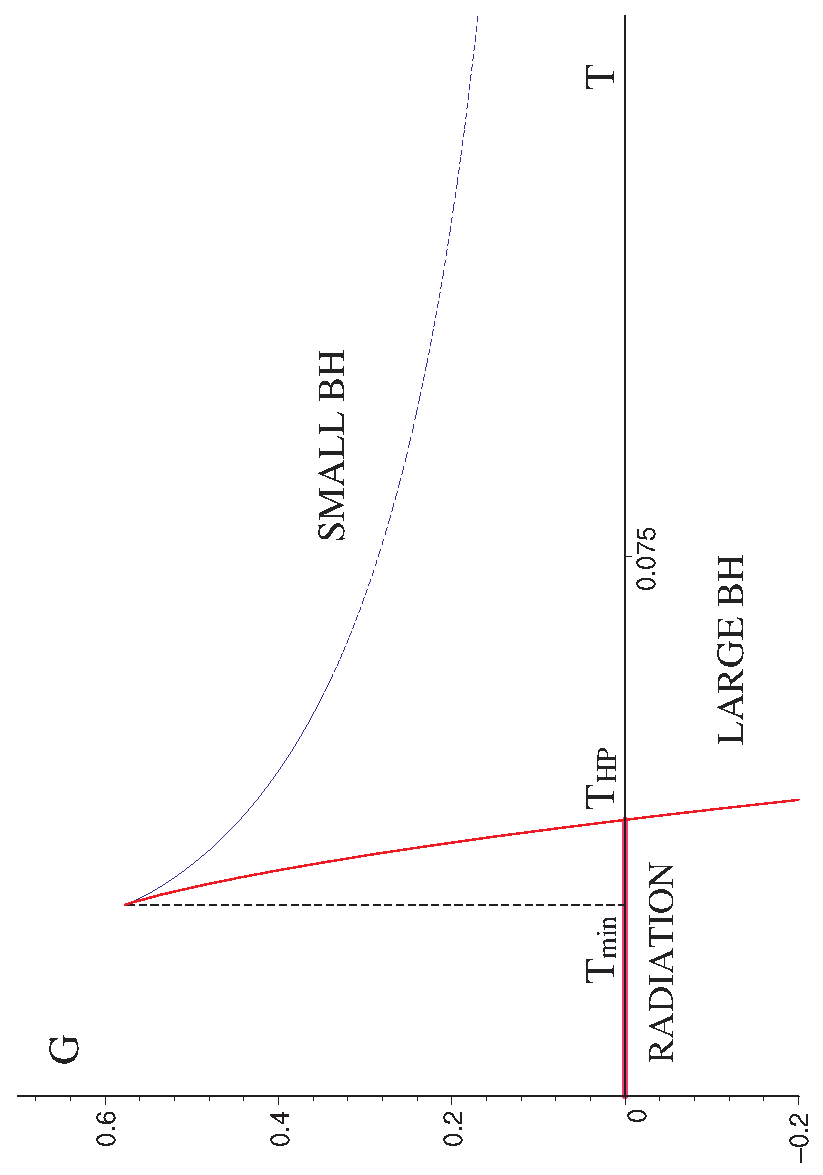
\includegraphics[width=0.4\textwidth,height=0.3\textheight]{Figures/HPG.eps}
}
\caption{{\bf Gibbs free energy: Schwarzchild-AdS black hole.}
When compared to the asymptotically flat Schwarzschild case (fig.~\ref{Fig:Gschflat}) for $P>0$ the Gibbs free energy acquires a new thermodynamically stable branch 
of large black holes. For $T>T_{\mbox{\tiny  HP}}$ this branch has negative Gibbs free energy and the corresponding black holes represent the 
globally thermodynamically preferred state. 
}
\label{Fig:Gschads}
\end{center}
\end{figure}

We observe a qualitatively different thermodynamic behaviour when compared to the asymptotically flat Schwarzschild case. Specifically $C_P$ is no longer always negative: it becomes positive for large (when compared to the AdS radius) black holes
\be
r_+>r_{\mbox{\tiny  min}}=\frac{l}{\sqrt{3}}\,,
\ee
while it is negative for $r_+<r_{\mbox{\tiny  min}}$ and ill defined at $r_+=r_{\mbox{\tiny  min}}$.




The behaviour of the Gibbs free energy $G$ is displayed in fig.~\ref{Fig:Gschads}.
We observe a minimum temperature $T_{\mbox{\tiny  \tiny min}}=2\sqrt{3}/(4\pi l)$, corresponding to $r_{\mbox{\tiny  min}}$, below which no black holes can exist. Above this temperature we have two branches of black holes. The upper one describes small (Schwarzschild-like) black holes with negative specific heat; these are thermodynamically unstable and  cannot be in a thermal equilibrium with a thermal bath of radiation. The large ($r_+>r_{\mbox{\tiny  \tiny min}}$) black holes at lower branch have positive specific heat and hence are locally thermodynamically stable. However, just above $T_{\mbox{\tiny  \tiny min}}$ the Gibbs free energy of such black holes is positive and the thermal AdS space with approximately zero Gibbs free energy represents a globally preferred thermodynamic state.\footnote{We refer to a thermal AdS space to be a (global) AdS space coupled to a bath of thermal radiation. Since the number of particle quanta representing the radiation is relatively small, the corresponding Gibbs free energy approximately equals zero.}     
This continues until temperature $T_{\mbox{\tiny  HP}}\approx 1/(\pi l)$ for which the black hole Gibbs free energy becomes negative, with the corresponding black hole radius given by 
\be
r_{\mbox{\tiny  HP}}=l\,.
\ee
Black holes with $r_+> r_{\mbox{\tiny  HP}}$ have negative Gibbs free energy and represent the globally preferred state. 
This means that at $T=T_{\mbox{\tiny  HP}}$ there is a first order {\em Hawking--Page} \cite{HawkingPage:1983} phase transition between thermal radiation and large black holes. This phase transition 
can be interpreted as a confinement/deconfinement phase transition in the dual quark
gluon plasma \cite{Witten:1998b}. 



Considering an extended phase space, the coexistence line of thermal radiation/large black hole phases, determined from $G=0$,
reads 
\be\label{HPcoexistence}
P|_{\mbox{\tiny  coexistence}}=\frac{3\pi}{8} T^2\,.
\ee
The corresponding $P-T$ phase diagram is displayed in fig.~\ref{Fig:HPtrans}.    
\begin{figure}
\begin{center}
\rotatebox{-90}{
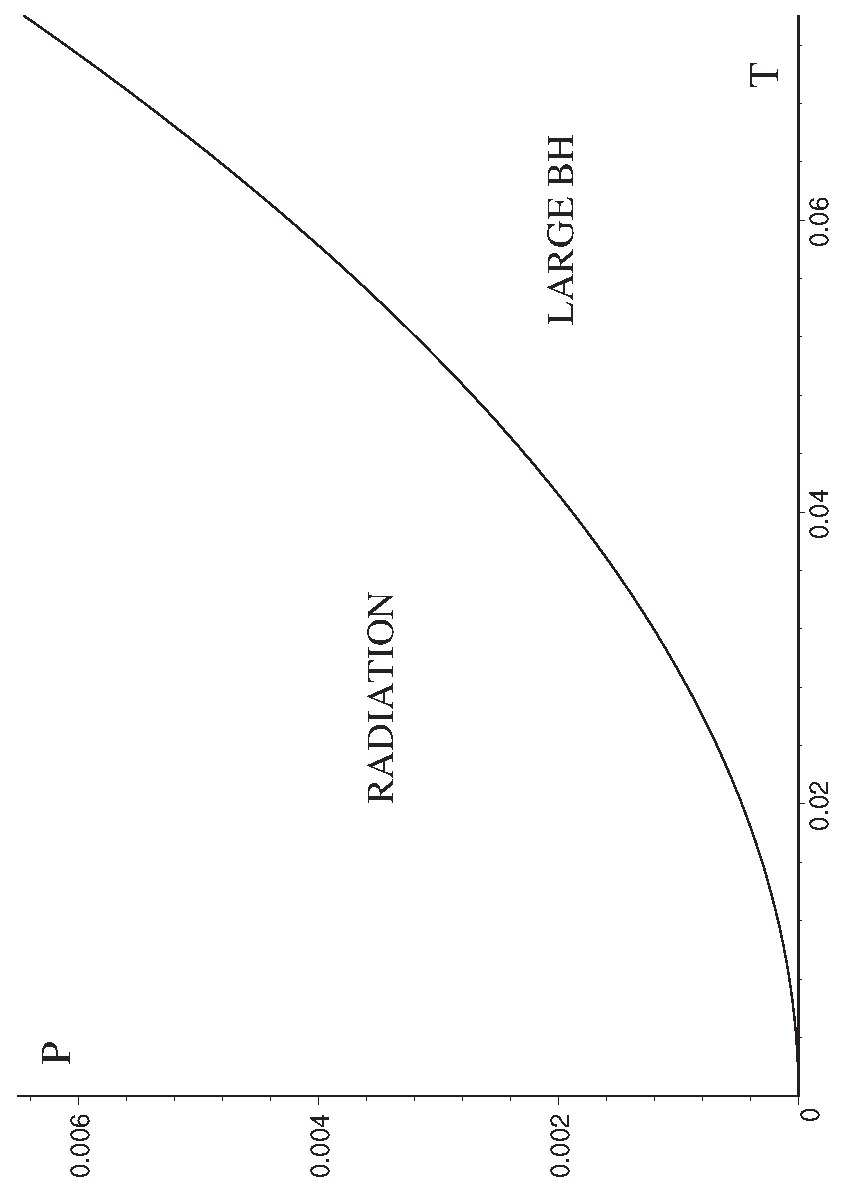
\includegraphics[width=0.4\textwidth,height=0.3\textheight]{Figures/HPtransition.eps}
}
\caption{{\bf Hawking--Page transition} is a first-order phase transition between thermal radiation in AdS and large stable Schwarzschild-AdS black hole. It occurs when $G$ of the Schwarzschild-AdS black hole approximately vanishes. Considering various pressures $P$ gives the radiation/large black hole coexistence line \eqref{HPcoexistence}  displayed in this figure. Similar to a ``solid/liquid'' phase transition, this line continues all the way to infinite pressure and temperature. 
}
\label{Fig:HPtrans}
\end{center}
\end{figure}


\begin{figure}
\begin{center}
\rotatebox{-90}{
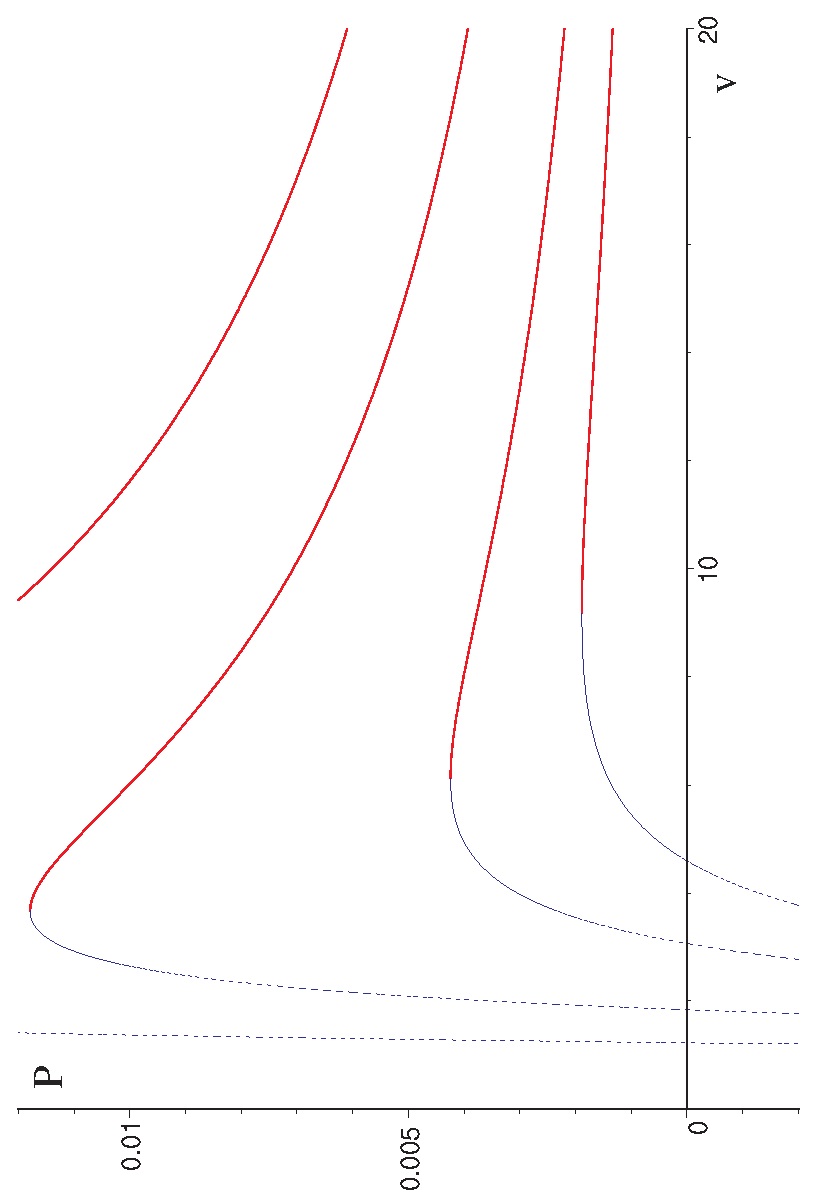
\includegraphics[width=0.4\textwidth,height=0.3\textheight]{Figures/HPstate.eps}
}
\caption{{\bf Equation of state: Schwarzschild-AdS black hole}. The equation of state \eqref{HPstate} is displayed for various temperatures. 
For a given temperature the maximum occurs at $v=2r_0$. The dashed blue curves correspond to small unstable black holes. The red curves depict the stable large black hole branch; we observe   `ideal gas' behaviour for large temperatures. 
}
\label{Fig:PVSchwAdS}
\end{center}
\end{figure}
By rewriting the temperature equation \eqref{SchaAdS} while using \eqref{PLambda}, we get a corresponding `fluid equation of state' 
for the Schwarzschild-AdS black hole, given by 
\be\label{HPstate}
P=\frac{T}{v}-\frac{1}{2\pi v^2}\,,\quad v=2\Bigl(\frac{3V}{4\pi}\Bigr)^{1/3}=2r_+\,.
\ee     
 The behaviour of this equation is displayed in the $P-V$ diagram in fig.~\ref{Fig:PVSchwAdS}. For each isotherm there is a maximum which occurs for $v=1/(\pi T)$. For a given temperature this precisely corresponds to $r_+=r_{\mbox{\tiny  \tiny min}}$; 
the dashed blue curves with positive slope (and possibly negative pressures) to the left of the maximum correspond to small black holes with negative $C_P$ which are thermodynamically unstable, whereas solid red curves correspond to large black holes with positive $C_P$ that are locally thermodynamically stable.



Let us compare the fluid equation of state of the Schwarzschild-AdS black hole \eqref{HPstate} with the famous {\em Van der Waals (VdW) equation}, e.g. \cite{Goldenfeld:1992},  which is a popular two parameter closed form modification of the ideal gas law that approximates the behaviour of real fluids. The VdW equation takes into account the nonzero size of fluid molecules 
(described by a constant $b>0)$ and the attraction between them (described by a constant $a>0$) and is often used to capture basic qualitative features of the liquid--gas phase transition. The equation reads (setting the Boltzmann constant $k_B=1$)
\be\label{VdW}
P=\frac{T}{v-b}-\frac{a}{v^2}\,,
\ee
where $v=V/N$ is the specific volume of the fluid, $P$ its pressure, $T$ its temperature, and the fluid parameters $a$ and $b$ are characteristics 
of a given fluid. The characteristic VdW $P-v$ diagram is displayed in fig.~\ref{fig:PVVdWstate}.
The equation admits a critical point, described by $\{T_c, v_c, P_c\}$, with universal critical ratio 
\be\label{universalVdWratio}
\rho_c=\frac{P_c v_c}{T_c}=\frac{3}{8}\,,
\ee
and the mean field theory critical exponents \eqref{MFT}.
\begin{figure}\label{fig:Fig1}
\begin{center}
\rotatebox{-90}{
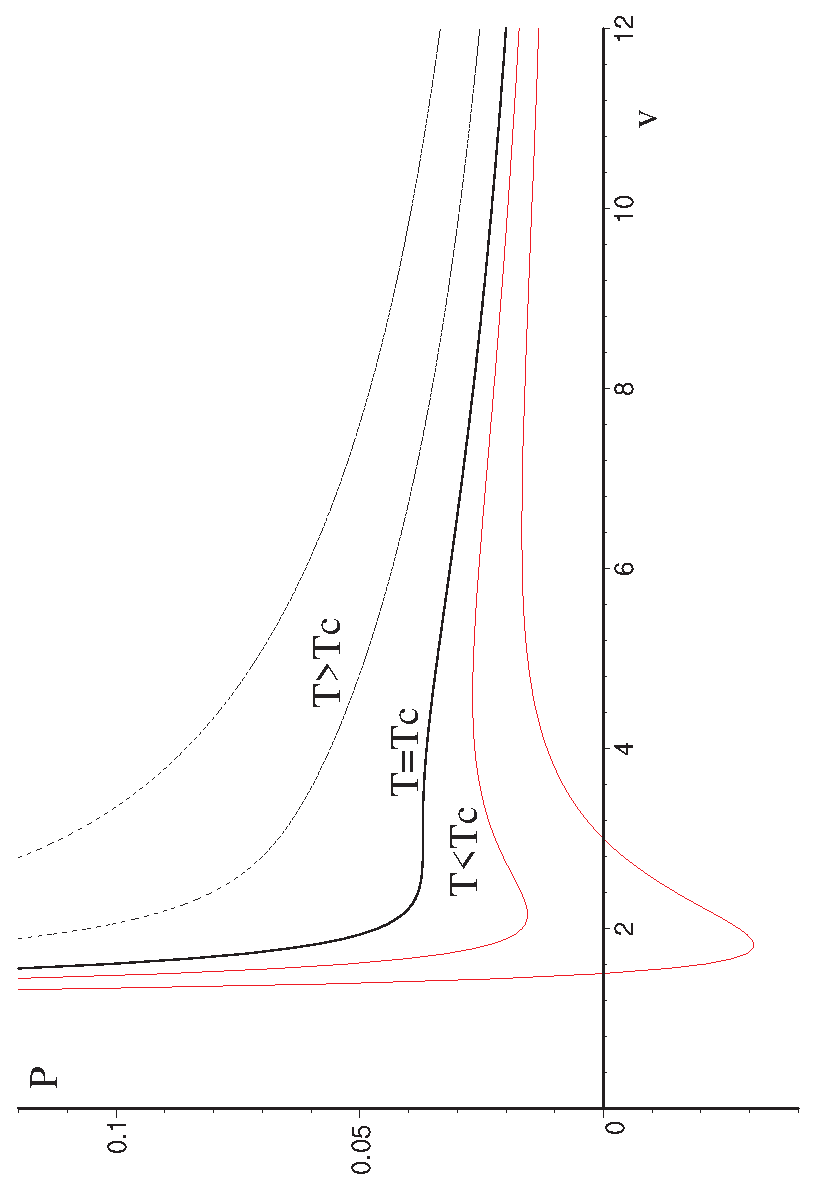
\includegraphics[width=0.39\textwidth,height=0.32\textheight]{Figures/PVVdW.eps}
}
\caption{{\bf $P-v$ diagram of Van der Waals fluid.} The temperature of isotherms decreases from top to bottom. The two upper dashed lines correspond to the ``ideal gas'' phase for $T>T_c$, the critical isotherm $T=T_c$ is denoted by the thick solid line, lower solid lines correspond to temperatures smaller than the critical temperature; for $T<T_c$ parts of the isotherms are actually unphysical, and must be replaced by a constant pressure line according to the Maxwell's equal area prescription \cite{KubiznakMann:2012}. Constants $a$ and $b$ were set equal to one.  
}  \label{fig:PVVdWstate}
\end{center}
\end{figure} 

We pause to consider topological Schwarzschild-AdS black holes.  Making use of the metric \eqref{ss} for arbitrary $k$, the 
formulae \eqref{SchaAdS} take the following more general form:
\ba
M &=& \frac{r_+ A_k}{8}\Bigl(k + \frac{r^2_+}{\ell^2}\Bigr)\,, \quad S=\frac{\pi A_k}{4} r^2_+\,, \nonumber\\
T &=& \frac{k \ell^2 + 3r^2_+}{4\pi\ell^3 r_+}\,,\quad V = \frac{\pi A_k}{3} r^3_+ \,,
\ea
where  $A_k$ is the area of the constant-curvature space divided by $\pi$; for a sphere, $A_{k=1} = 4$, 
for a torus, $A_{k=0} = A B$, where $A$ and $B$ and the sides of the torus, and there is no nice simple formula for $A_{k=-1}$.
In all cases the Smarr formula \eqref{Smarr} and first law \eqref{1st} hold.
It is then straightforward to show that the fluid corresponding to the  Schwarzschild-AdS black hole is characterized by
\be
a=\frac{k}{2\pi}\,,\quad b=0\,.
\ee
That is, its equation of state differs from the ideal gas law by the presence of a nontrivial parameter $a=k/(2\pi)$. This is directly related to the  topology of the horizon. For {\em planar} Schwarzschild-AdS black holes, $k=0$ and we recover the ideal gas law characterized by $a=0=b$, 
\be
Pv=T\,,
\ee
whereas for the $k=-1$ hyperbolic case we get a peculiar `repulsion' feature $a=-\frac{1}{2\pi}<0$, with $b=0$, the volume of molecules still vanishing.

We note one more interesting fact  for the planar ($k=0)$ AdS black holes.   In this case the following specific Smarr-like relation has been employed  e.g., \cite{Bertoldi:2010ca,Berglund:2011cp}:
\be\label{differentSmarr}
3 M=  2 TS\,,
\ee
[or $(d-1) M=(d-2) TS$ in  $d$-dimensions] without any reference to the $PV$ term. 
The value of our  Smarr relation \eqref{Smarr} is that it follows from the general geometric argument and 
applies to a wide class of (even possibly unknown) solutions that satisfy the assumptions of the theorem, whereas \eqref{differentSmarr} is a `phenomenological' observation valid for a particular sub-class of solutions. We also note that this relation is not related to the corresponding 
first law, $dM=TdS$, by a dimensional scaling argument.


 \subsection{Reissner–Nordstrom Solution}
 The charged AdS black hole metric is described by \eqref{ss} with
\be
f=1-\frac{2M}{r}+\frac{Q^2}{r^2}+\frac{r^2}{l^2}\,.
\ee
The thermodynamic quantities are 
\ba
T&=&\frac{1}{4\pi r_+^3 l^2}\Bigl(l^2(r_+^2-Q^2)+3r_+^4\Bigr)\,,\quad S=\pi r_+^2\,,\nonumber\\
V&=&\frac{4}{3}\pi r_+^3\,,\quad \Phi=\frac{Q}{r_+}\,,\quad 
G=\frac{l^2r_+^2-r_+^4+3Q^2l^2}{4l^2r_+}\,,\nonumber\\
C_P&=&2\pi r_+^2\frac{3r_+^4+l^2r_+^2-Q^2l^2}{3r_+^4-l^2r_+^2+3Q^2l^2}\,.
\ea
The specific heat is negative for 
\be
\frac{l \sqrt{1-\sqrt{1-36Q^2/l^2}}}{\sqrt{6}}<r_+<\frac{l \sqrt{1+\sqrt{1-36Q^2/l^2}}}{\sqrt{6}}\,,
\ee
and positive otherwise.


\begin{figure}
\begin{center}
\rotatebox{-90}{
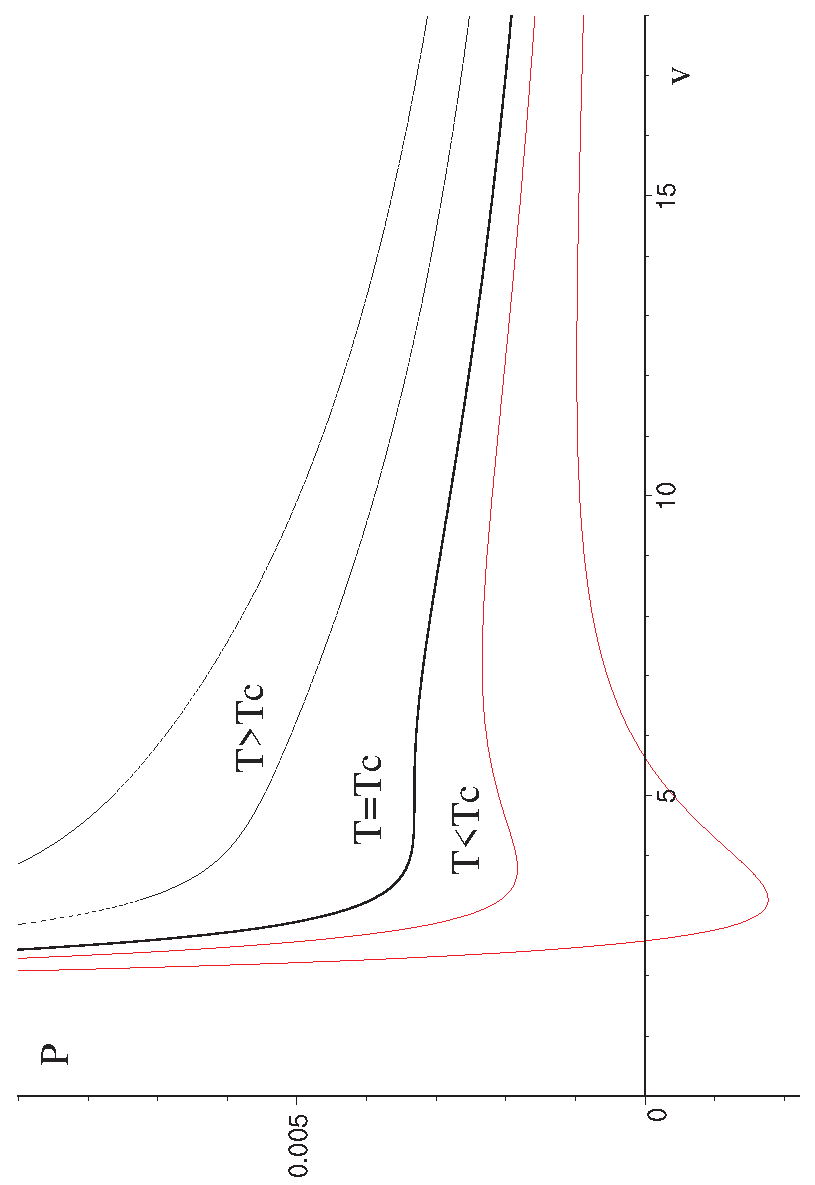
\includegraphics[width=0.39\textwidth,height=0.34\textheight]{Figures/rP.eps}
}
\caption{{\bf Equation of state: charged AdS black hole.}
The temperature of isotherms decreases from top to bottom. The two upper dashed lines correspond to the ``ideal gas'' one-phase behaviour for $T>T_c$, the critical isotherm $T=T_c$ is denoted by the thick solid line, lower solid lines correspond to temperatures smaller than the critical temperature.  We have set $Q=1$.  
$P-v$ diagram for the Kerr-AdS black hole with $J=1$ is qualitatively similar.
}\label{Fig:RNstate}
\end{center}
\end{figure} 
It was first noticed in \cite{ChamblinEtal:1999a,ChamblinEtal:1999b} that in a canonical (fixed charge) ensemble, charged AdS black holes allow for a first order {\em small-black-hole/large-black-hole} phase (SBH/LBH) transition which is in many ways reminiscent of the liquid/gas transition of a Van der Waals fluid.
This analogy becomes more complete in extended phase space \cite{KubiznakMann:2012}. 
Namely, the equation of state,
\be\label{RNstate}
P=\frac{T}{v}-\frac{1}{2\pi v^2}+\frac{2Q^2}{\pi v^4}\,,\quad v=2r_+\,,
\ee
mimics qualitatively the behaviour of the Van der Waals equation, shown in fig. \ref{fig:PVVdWstate}, with its black hole counterpart \eqref{RNstate} illustrated in fig. \ref{Fig:RNstate}.
Below $P_c$, the Gibbs free energy displays a characteristic swallowtail behaviour, depicted in fig.~\ref{Fig:Grnads}, indicating a first-order SBH/LBH phase transition. The corresponding coexistence line is displayed in fig.~\ref{Fig:RNPT}. 
It terminates at a critical critical point, characterized by 
\be
T_c=\frac{\sqrt{6}}{18\pi Q}\,,\quad v_c=2\sqrt{6} Q\,,\quad P_c=\frac{1}{96\pi Q^2}\,, 
\ee
where the phase transition becomes of the second order \cite{Banerjee:2010bx, MoLiu:2013}, and is characterized by the mean field theory critical exponents \eqref{MFT}. Remarkably the relation $\rho_c=P_c v_c/T_c=3/8$ is identical to  the Van der Waals case. The overall situation reminds one of the liquid/gas phase transition.  
A similar situation occurs for charged AdS black holes in higher dimensions \cite{GunasekaranEtal:2012}. 
\begin{figure}
\begin{center}
%\rotatebox{-90}{
\includegraphics[width=0.4\textwidth,height=0.3\textheight]{Figures/GrnAdS.eps}
%}
\caption{{\bf Gibbs free energy: charged AdS black hole.}
Characteristic swallowtail behaviour is observed for $P<P_c$, corresponding to a small/large black hole phase transition.
An unstable branch of the Gibbs free energy is displayed in dashed blue line. We have set $Q=1$.
The behaviour of $G$ for Kerr-AdS black hole with $J=1$ is qualitatively similar.
}
\label{Fig:Grnads}
\end{center}
\end{figure}
\begin{figure}
\begin{center}
\rotatebox{-90}{
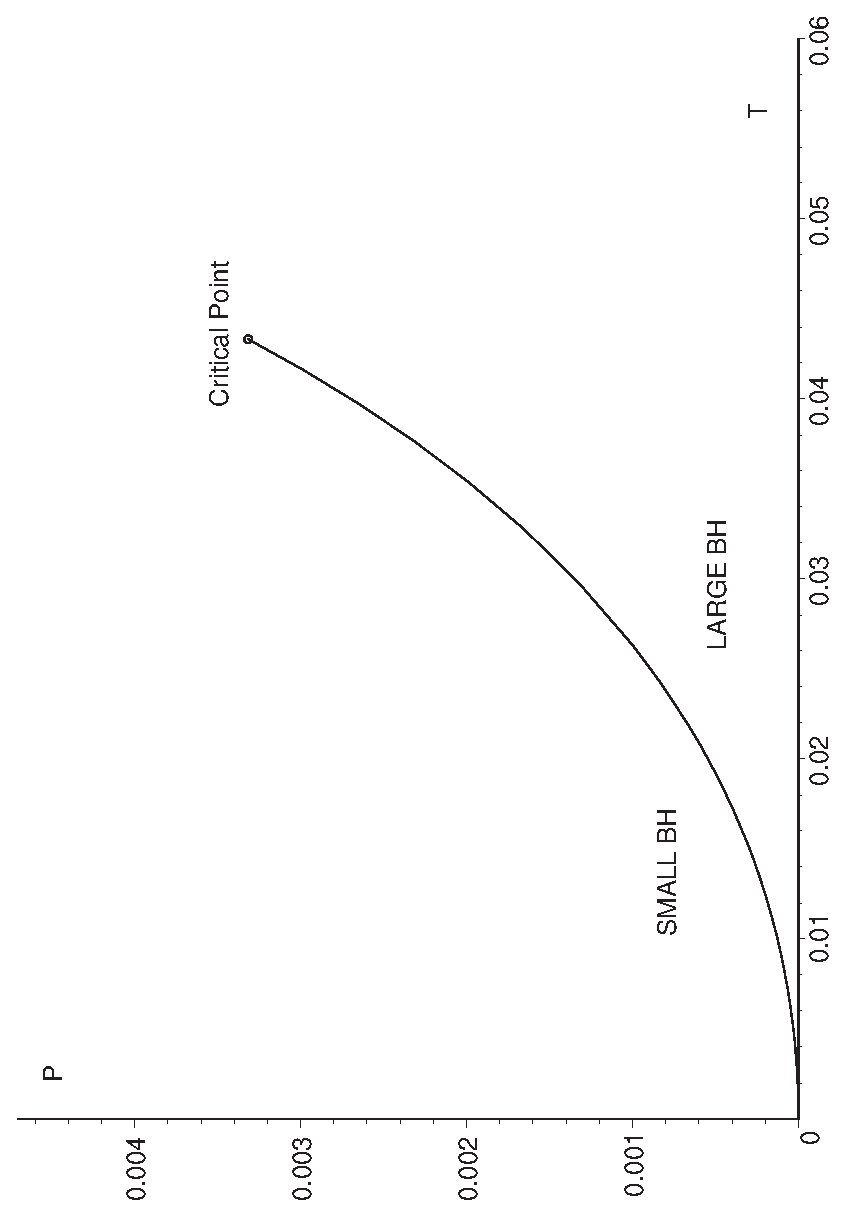
\includegraphics[width=0.39\textwidth,height=0.34\textheight]{Figures/PT2.eps}
}
\caption{{\bf Phase diagram: charged AdS black hole.} The coexistence line of the SBH/LBH phase transition of the charged AdS black hole system in $(P, T)$-plane is displayed. The critical point is highlighted by a small circle at the end of the coexistence line. The
phase diagram for a Kerr-AdS black hole with $J=1$ is qualitatively similar.
} \label{Fig:RNPT} 
\end{center}
\end{figure} 

We remark that the Hawking--Page phase transition as well as the SBH/LBH phase transition ala Van der Waals can be also observed for asymptotically flat or de Sitter charged black holes provided these are placed in a finite cavity \cite{Carlip:2003ne}.  



We close this subsection by noting that strongly charged small AdS black holes are subject to superradiant instabilities. For a charged scalar field coupled to Einstein--Maxwell theory a similar situation occurs:  
at small temperatures  charged scalar hair forms and the resulting `hairy black holes' are thermodynamically preferred  \cite{Gubser:2008px, Hartnoll:2008vx, Hartnoll:2008kx, Maeda:2010hf, Basu:2010uz, Dias:2011tj, Horowitz:2010gk, Hartmann:2013nla}. This means that in the presence of a charged scalar field, the left-most branch of small black holes in the Gibbs free diagram \ref{Fig:Grnads}, although locally thermodynamically stable, does not globally minimize the Gibbs free energy. Rather, there is another branch of hairy black holes with 
lower Gibbs free energy. The hair/no-hair black hole phase transition is of the second order and underlies the theory of holographic superconductors.   

  

 \subsection{Kerr Solution}
 
 
The thermodynamics of four-dimensional rotating AdS black holes is qualitatively similar to the charged AdS case.\footnote{In fact a qualitatively similar behaviour occurs for charged rotating AdS black holes, see \cite{CaldarelliEtal:2000}.} 
The metric is  
\begin{eqnarray}
ds^2&=&-\frac{\Delta}{\rho^2}(dt-\frac{a}{\Xi}\sin^2\!\theta d\varphi)^2+
\frac{\rho^2}{\Delta}dr^2+\frac{\rho^2}{\Sigma}d\theta^2 \nonumber \\
&+&
\frac{\Sigma \sin^2\!\theta}{\rho^2}[adt-\frac{(r^2+a^2)}{\Xi}d\varphi]^2\,,
\end{eqnarray}
where
\begin{eqnarray}
\Delta&=&(r^2+a^2)(1+\frac{r^2}{l^2})-2mr\,,\quad
\Sigma=1-\frac{a^2}{l^2}\cos^2\theta \,,\nonumber \\
\Xi&=&1-\frac{a^2}{l^2}\,, \quad
\rho^2=r^2+a^2\cos^2\theta \,. \nonumber
\end{eqnarray}
The thermodynamic quantities read 
\begin{eqnarray}
M&=&\frac{m}{\Xi^2}\,, \quad J=\frac{ma}{\Xi^2} \,, \quad  \Omega=\frac{a}{l^2}\frac{r_+^2+l^2}{r_+^2+a^2}\,, \nonumber\label{OHJ}\\
T&=&\frac{1}{2\pi r_+}\Bigr[\frac{(a^2+3r_+^2)(r_+^2/l^2+1)}{2(a^2+r_+^2)}-1\Bigr]\,, \nonumber\label{BHT} \\
S &=&\pi \frac{(a^2+r_+^2)}{\Xi}=\frac{A}{4} \,,\quad V=\frac{r_+A}{3}\Bigl(1+\frac{1+r_+^2/l^2}{2r_+^2}\frac{a^2}{\Xi}\Bigr)\,, \nonumber\label{BHS}\\
G &=& \frac{(r^2_+ + 3a^2) l^4 -(r^2_+ - a^2)^2 l^2 + (a^2 + 3 r^2_+)a^2 r^2_+}{l^4 \Xi^2 r_+}\,, \nonumber \\
\end{eqnarray}
and satisfy the Smarr relation \eqref{Smarr}; 
rather lengthy formula for $C_P$ can be found in \cite{MonteiroEtal:2009}.
%\ba
%C_P=-\frac{2\pi l^4(a^2+r_+^2)^2[(r_+^2-l^2)a^2+r_+^2(l^2+3r_+^2)]}
%{(a^2-l^2)[(3a^4+6r_+^2a^2-r_+^4)l^4+(a^6+13r_+^2a^4+23r_+^4a^2+3r_+^6)l^2
%+a^2r_+^2(a^2+3r_+^2)^2]}\,.
%\ea

The Gibbs free energy, equation of state, and the $P-T$ phase diagram are qualitatively similar to figs.~\ref{Fig:Grnads}, \ref{Fig:RNstate} and 
\ref{Fig:RNPT}---with fixed $J$ replacing fixed $Q$.  For any fixed $J$, there is a critical point, characterized by $(P_c, V_c, T_c)$, that can be determined numerically. For $P<P_c$, the Gibbs free energy displays  swallowtail behaviour and there is a corresponding SBH/LBH first order phase transition with a phase diagram similar to fig.~\ref{Fig:RNPT}. It will be shown in the next section that in the limit of slow rotation,  $a\ll l$, the equation of state can be approximated by 
\ba
P&=&\frac{T}{v}-\frac{1}{2\pi v^2}+\frac{48J^2}{\pi v^6}-\frac{384 J^4(7+8\pi Tv)}{(1+\pi Tv)^2\pi v^{10}}\nonumber\\
&&+\frac{36864(13\pi Tv\!+\!11)J^6}{\pi v^{14}(1+\pi Tv)^3}\!+\!O\bigl[(a/l)^8\bigr]\,,\nonumber \\
v&=&2\Bigl(\frac{3V}{4\pi}\Bigr)^{\!1/3}\,.
\ea
The first three terms were first obtained in \cite{GunasekaranEtal:2012}. Using this equation of state, one can approximately find 
the critical point and study its characteristics. In particular, one finds that the critical exponents 
remain as predicted by the mean field theory, given by \eqref{MFT}. 

We pause to remark that, similar to the charged AdS case, the rotating AdS black holes close to extremity are unstable with respect to   superradiant instabilities;  the resultant objects (hairy black hole, soliton, or boson star) are expected to globally minimize the Gibbs free energy \cite{Hawking:1999dp, Sonner:2009fk, Dias:2010ma, Cardoso:2013pza}.




 \subsection{general solution }
 
 
 \subsection{Higher-dimensional Kerr-AdS black hole spacetimes}
General Kerr-AdS black hole spacetimes \cite{GibbonsEtal:2004, GibbonsEtal:2005}  are $d$-dimensional metrics that solve the Einstein equations with  cosmological constant
\be
R_{ab} =\frac{2\Lambda}{(d-2)}  g_{ab}
\ee
and generalize the $d$-dimensional asymptotically-flat rotating black hole spacetimes of Myers and Perry \cite{MyersPerry:1986}.   
In   Boyer--Lindquist  coordinates the metric takes the form
\ba \label{metric}
ds^2&=&-W\Bigl(1+\frac{r^2}{l^2}\Bigr)d\tau ^2+\frac{2m}{U} \Bigl(W d\tau -\sum_{i=1}^{N} \frac{a_i \mu_i ^2 d\varphi _i}{\Xi _i}\Bigr)^2\nonumber\\
&+&\sum_{i=1}^{N} \frac{r^2+a_i^2}{\Xi _i} \mu_i ^2 d\varphi _i^2+\frac{U dr^2}{F-2m}+\sum_{i=1}^{N+\varepsilon}\frac{r^2+a_i ^2}{\Xi _i} d\mu _i ^2 \nonumber\\
&-&\frac{l^{-2}}{W (1+r^2/l^{2})}\Bigl(\sum_{i=1}^{N+\varepsilon}\frac{r^2+a_i ^2}{\Xi _i} \mu_i d\mu_i\Bigr)^2\,,
\ea
where 
\ba\label{metrcifunctions}
W&=&\sum_{i=1}^{N+\varepsilon}\frac{\mu _i^2}{\Xi _i}\,,\quad U=r^\varepsilon \sum_{i=1}^{N+\varepsilon} \frac{\mu _i^2}{r^2+a_i^2} \prod _j ^N (r^2+a_j^2)\,,\nonumber\\
F&=&r^ {\varepsilon -2} \Bigl(1+\frac{r^2}{l^2}\Bigr) \prod_{i=1}^N (r^2+a_i^2)\,,\quad \Xi_i=1-\frac{a_i^2}{l^2}\,.\quad
\ea
To treat even ($\varepsilon=1)$  odd ($\varepsilon=0)$ spacetime dimensionality $d$ simultaneously, we have parametrized
\be
d=2N + 1 + \varepsilon\,,
\ee 
and in even dimensions set for convenience $a_{N+1}=0$.
The  coordinates $\mu_i$ are not independent, but obey the constraint
\begin{equation}\label{constraint}
\sum_{i=1}^{N+\varepsilon}\mu_i^2=1\,.
\end{equation}
In general the spacetime admits $N$ independent angular momenta $J_i$, described by
$N$ rotation parameters $a_i$, and generalizes the previously known singly-spinning case \cite{HawkingEtal:1999}.
In $d=4$ it reduces to the four-dimensional Kerr-AdS metric studied in the previous section.  
With this metric it shares a remarkable property---it possesses a hidden symmetry associated with the Killing--Yano tensor \cite{KubiznakFrolov:2007} that is responsible for integrability of geodesic motion and various test field equations in these spacetimes, see, e.g., review \cite{FrolovKubiznak:2008}.

 

The thermodynamic quantities associated with Kerr-AdS black holes were first calculated in \cite{Gibbons:2004ai}.
The mass $M$, the angular momenta $J_i$, and the angular velocities of the horizon $\Omega_i$ read
\ba \label{TD}
M&=&\frac{m \omega _{d-2}}{4\pi (\prod_j \Xi_j)}\bigl(\sum_{i=1}^{N}{\frac{1}{\Xi_i}-\frac{1-\varepsilon }{2}}\bigr)\,,\nonumber\\
J_i&=&\frac{a_i m \omega _{d-2}}{4\pi \Xi_i (\prod_j \Xi_j)}\,,\quad \Omega_i=\frac{a_i (1+\frac{r_+^2}{l^2})}{r_+^2+a_i^2}\,,
\ea
while the temperature $T$, the horizon area $A$, and the entropy $S$ are given by
\ba\label{TS}
T&=&\frac{1}{2\pi }\Bigr[r_+\Bigl(\frac{r_+^2}{l^2}+1\Bigr)
\sum_{i=1}^{N} \frac{1}{a_i^2+r_+^2}-\frac{1}{r_+}
\Bigl(\frac{1}{2}-\frac{r_+^2}{2l^2}\Bigr)^{\!\varepsilon}\,\Bigr]\,,\nonumber\\
A&=&\frac{\omega _{d-2}}{r_+^{1-\varepsilon}}\prod_{i=1}^N 
\frac{a_i^2+r_+^2}{\Xi_i}\,,\quad S=\frac{A}{4}\,. 
\ea
The horizon radius $r_+$ is determined as the largest root of $F-2m=0$ and $\omega_{d}$ is given by \eqref{omega}.


The thermodynamic volume reads \cite{CveticEtal:2010, Dolan:2013}
\begin{eqnarray} \label{VBHKerr}
V& =& \frac{r_+ A }{d-1}\left[1+\frac{1+{r^2_+}/{l^2}}{(d-2)r_+^2}\sum_i \frac{a_i^2}{\Xi_i}\right]  \nonumber\\ \label{VBHKerr2}
&=&	{\frac{r_+ A }{d-1}+{8\pi\over (d-1)(d-2)}\sum_i a_iJ_i }\,, 
\end{eqnarray}
and indeed is required to ensure that the Smarr formula \eqref{Smarr} holds.
It is known to obey the {\em reverse isoperimetric inequality} \eqref{ISO} provided that in \eqref{ratio} we identify ${\cal A}=A$ and ${\cal V}=V$
as given by \eqref{TS} and \eqref{VBHKerr}.
In fact the inequality is saturated for non-rotating black holes, whereas it becomes most extreme $({\cal R}\to \infty)$
in the ultraspinning limit, see discussion around Eq. \eqref{ratioInfinity}.


Note that the `naive' {\em geometric volume} \cite{Parikh:2006, BallikLake:2010, CveticEtal:2010,BallikLake:2013} (given by the spatial integral of $\sqrt{-g}$ integrated up to the horizon radius) 
\be
V'=\frac{r_+ A}{d-1}\,
\ee
and the thermodynamic volume $V$ in \eqref{VBHKerr} differ by an $\sum_i a_iJ_i$ term and behave differently in the limits of slow and fast rotation. 
Whereas the thermodynamic volume \eqref{VBHKerr} is dominated by its first geometric term for slow rotations 
\be\label{Vslow}
V_{\mbox{\tiny  slow}}\approx V'_{\mbox{\tiny  slow}}\approx\frac{\omega_{d-2}r_+^{d-1}}{d-1}\,,
\ee
in the ultraspinning regime the second (angular momentum) term dominates.
To see this let us, for simplicity, consider for a moment 
a singly spinning Myers--Perry black hole ($a_1=a$, other $a_i=0$, and $l\to \infty$). 
In this case the formula \eqref{VBHKerr} reduces to  the following expression 
\be\label{VKerr}
V=V'+\frac{4\pi}{d-1}\frac{J^2}{M}
\ee
which is also valid for the $d=4$ Kerr-AdS case.
In $d\geq 6$ there is no limit on how large the rotation parameter $a$ can be \cite{EmparanMyers:2003} and one can, in principle, take the {\em ultraspinning limit} $a\to \infty$. For fixed $M$ this implies $r_+\to 0$, and the second term in the previous formula dominates.
Hence, for the ultraspinning black holes, the thermodynamic volume differs significantly from the geometric one, being approximately given by
\be\label{VeqV'}
V\approx \frac{4\pi}{d-1}\frac{J^2}{M}\approx \frac{\omega_{d-2} a^4 r_+^{d-5}}{(d-1)(d-2)}\,,
\ee
which is to be compared with formula \eqref{Vslow}. The conclusions for multiply-spinning and/or AdS black holes are   analogous.

The Gibbs free energy is given by \eqref{G} and is related to the Euclidean action $I$ \cite{Gibbons:2004ai},  
\be\label{action}
I=\frac{\omega_{d-2}}{8\pi T\bigl(\prod_j \Xi_j\bigr)}\Bigl(m-\frac{r_+^\varepsilon}{l^2}\prod_{i=1}^N(r_+^2+a_i^2)\Bigr)\,,
\ee
by 
\be\label{GibbsKerrAdS}
G=M-TS=TI+\sum_{i}\Omega_i J_i\,,
\ee
see also Sec.~\ref{sec:Instab} where $I$ is used to estimate the onset of ultraspinning instabilities.  
In what follows we shall discuss in detail some special cases of these general metrics and the associated interesting thermodynamic features.


\section {Géométrie thermodynamique et transition de phase}

 Une autre approche pour étudier le comportement thermodynamique du système est la géométrie thermodynamique. Cette méthode nécessite une métrique appropriée en utilisant des quantités thermodynamiques. Pour construire une métrique appropriée, on peut utiliser un potentiel thermodynamique avec
ensemble spécifique de paramètres étendus. Puis en calculant le scalaire de Ricci de la métrique introduite
et en déterminant les points de divergence, on peut étudier les deux types de transition de phase. Il
a été démontré que le résultat obtenu est similaire au résultat de la capacité calorifique. Ça veut dire
les points de divergence du scalaire de Ricci et la divergence / point zéro de la capacité thermique coïncident.\\
Comme mentionné en introduction, il existe plusieurs méthodes pour construire un espace-temps géométrique telles que
Métrique Weinhold, Ruppeiner, Quevedo et HPEM. Nous passons d'abord en revue les quatre mesures mentionnées
et étudiez la transition de phase du trou noir chargé en accélération AdS chargé dans une phase non étendue
espace et espace de phase étendu. Ensuite, nous comparerons les résultats avec la capacité thermique et
trouvera la métrique appropriée pour étudier la transition de phase d'un trou noir chargé en accélération AdS.\\
Comme mentionné, nous considérons la charge électrique comme un paramètre fixe dans la transition de phase
de la capacité thermique dans un ensemble canonique. Mais la construction d'une métrique thermodynamique peut constituer une variable considérable. Pour trou noir accéléré chargé en AdS dans un espace de phase non étendu,
nous supposons que la pression est une quantité thermodynamique fixe et considérons la masse totale comme
potentiel thermodynamique et l'entropie et la charge électrique comme paramètres étendus. À présent
nous voulons étudier la transition de phase du trou noir accéléré chargé en AdS par ce qui précède
métriques thermodynamiques mentionnées.

\subsection{Métrique de Weinhold et Ruppeiner}
La première formulation géométrique a été introduite par Weinhold\cite{52}. Il a défini la métrique thermodynamique
 comme la dérivée seconde de la masse (énergie interne) par rapport à l'entropie et
d'autres paramètres étendus. La métrique de Weinhold est donnée par,
\begin{equation}
g_{ij}^{w}=\dfrac{\partial^{2}M(x^{k})}{\partial x^{i} \partial x^{j} };  x^{i}=(S,N^{a}) 
\end{equation}

où S est l'entropie et $N^{a}$ détermine toutes les autres variables étendues du système.\\
Cette métrique de Weinhold est conforme à la métrique de Ruppeiner 
avec  la température comme facteur conforme
\begin{equation}
g_{ij}^{w}= T g_{ij}^{R}
\end{equation}

la métrique de Ruppeiner \cite{53} est définie comme la dérivée seconde de l’entropie par rapport à l’énergie
interne et d’autres variables extensives. La metrique de Ruppeiner est défini par,
\begin{equation}
\label{xss}
g_{ij}^{R}=-\dfrac{\partial^{2}S(x^{k})}{\partial x^{i} \partial x^{j} }=\dfrac{1}{T}\dfrac{\partial^{2}M(x^{k})}{\partial x^{i} \partial x^{j} };  x^{i}=(U,N^{a}) 
\end{equation}

où U est l'entropie et $N^{a}$ détermine les variables extensives du système.\\
Dans l'espace des états on considère $x^{\mu} = (S, Q)$ comme variables extensives. Un calcul simple de courbure de la métrique\ref{xss} donne
\begin{equation}
R=-\dfrac{1}{\sqrt{g}}\left[\dfrac{\partial}{\partial S}\left( \dfrac{g_{SQ}}{g_{SS}\sqrt{g}}\dfrac{\partial g_{SS}}{\partial Q}-\dfrac{1}{\sqrt{g}}\dfrac{\partial g_{QQ}}{\partial S}\right)  +\dfrac{\partial}{\partial Q}\left( \dfrac{2}{\sqrt{g}}\dfrac{\partial g_{SQ}}{\partial S}-\dfrac{1}{\sqrt{g}}\dfrac{\partial g_{QQ}}{\partial S}-\dfrac{1}{\sqrt{g}}\dfrac{\partial g_{SS}}{\partial Q}-\dfrac{g_{SQ}}{g_{SS}\sqrt{g}}\dfrac{\partial g_{SS}}{\partial S}\right)\right] 
\end{equation}
Danc n peut exprimer le scalaire de Ricci de la  métrique de Ruppeiner  comme
\begin{equation}
R^{R}=\dfrac{8PS(8PS^{2}+\pi Q^{2})(S(8PS-3)+3\pi Q^{2})}{(S(8PS-1)+\pi Q^{2})^{2}(\pi Q^{2}-S(8PS+1))}
\end{equation}
nous avons tracé le scalaire  Ricci  de Ruppeineren ce qui concerne l'entropie dans les figures suivants\\

\begin{figure}[H]
%\includegraphics[scale=0.8]{images/metriqueR.png}
\caption{La courbure scalaire de la géométrie de Ruppeiner pour une transition de phase
	de première ordre $P < P_{c}$ (à gauche) et de deuxième ordre où $P = P_{c}$ (à droite) . On fixe Q = 1.}
\end{figure} 

Nous pouvons remarquer que le point de divergence n’est pas identique à celui de la
capacité thermique $(S_{min}, S_{max})$ pour $P < P_{c}$ et Sc pour$ P = P_{c}$. Par conséquent,
c'est à dire 
que le point de divergence n'est pas identique à la divergence / point zéro de la capacité calorifique, c'est pourquoi
Métrique n'est pas en mesure de décrire la transition de phase de cette solution de trou noir.
\subsection{Métrique de Quevedo}
Comme nous le savons, la métrique de Ruppeiner et la métrique de Weinhold ne sont pas invariantes sous Legendre.
transformation. Pour cette raison, Quevedo a introduit une métrique invariante de Legendre,
dans l'espace de l'état d'équilibre \cite{54}. Le Quevedo a deux types de métriques correspondantes
qui sont donnés par \cite{55},

\begin{equation}
dS_{Q}^{2}=g{ij}^{Q}dx^{i}dx^{j},
\end{equation}

Or $g_{ij}^{Q}$ est donnée par 
\begin{equation}
g{ij}^{Q}=\left( S\dfrac{\partial M}{\partial S}+Q\dfrac{\partial M}{\partial Q}\right)
\begin{pmatrix}
 -\dfrac{\partial^{2}M}{\partial S^{2}}  & 0\\
  0                                     & \dfrac{\partial^{2}M}{\partial Q^{2}}                  
\end{pmatrix}
\end{equation}

le scalaire de Ricci de cette métrique est

\begin{equation}
R_{ij}^{Q}=\dfrac{32\pi^{2} S^{2}\left(9\pi^{2}Q^{4}(28PS-1)+3\pi Q^{2}S(4PS(16PS-5)+3)+8PS^{3}(4PS(1-40PS)+1) \right) }{\left(-8PS^{2}-3\pi Q^{2}+S \right)^{2}\left(8PS^{2}+3\pi Q^{2}+S \right)^{3}  }
\end{equation}

nous avons tracé le scalaire  Ricci  de Quevedoen ce qui concerne l'entropie dans les figures suivants \\

\begin{figure}[H]
%	\includegraphics[scale=0.8]{images/metriqueQ.png}
	\caption{La courbure scalaire de la géométrie de Quevedo pour une transition de phase
		de première ordre $P < P_{c}$ (à gauche) et de deuxième ordre où $P = P_{c}$ (à droite) . On fixe Q = 1.}
\end{figure}

Il est clair que cette métrique présente des points de divergence qui coïncident avec
ceux de la capacité thermique. On peut dire que cette géométrie est capable de décrire la
transition de phase 1er/2ème ordre pour les trous noirs de RN-AdS.

\subsection{Métrique de Hendi, Panahiyan et Eslam HPEM}
En 2015 Hendi et ses collaborateurs ont introduit une nouvelle métrique \cite{56} qui contenait les deux types de transition de phase. C’est un métrique qui rectifie les lacunes de la
géométrie de Ruppeiner et Quevedo. La géométrie de HPEM est donnée par
\begin{equation}
g_{ij}^{HPEM}=\left( \dfrac{S M_{s}}{M_{QQ}^{3}}\right)
\begin{pmatrix}
-M_{SS}  & 0\\
0        & M_{QQ}
\end{pmatrix}
\end{equation}

Calculant le sclaire de HPEM Ricci,son dénominateur est 
\begin{equation}
demn(R_{HPEM})=S^{3}M_{S}^{3}M_{SS}^{2}
\end{equation}

On trace le scalir Ricci de HPEM  en fonction de l'entropie\\

\begin{figure}[H]
%	\includegraphics[scale=0.8]{images/matriqueH.png}
	\caption{La courbure scalaire de la géométrie de HPEM pour une transition de phase
		de première ordre $P < P_{c}$ (à gauche) et de deuxième ordre où $P = P_{c}$ (à droite) . On fixe Q = 1.}
\end{figure}

On peut voir que les points de divergence coïncident exactement avec les points de
divergence de la capacité calorifique ainsi que son point zéro. Alors on peut dire que cette
métrique peut décrire la transition de phase et déterminer le trou noir extrémal donné
par $C_{p} = 0$ ou T = 0.\\
\\
En étudiant la géométrie thermodynamique dans l'espace de phase, on remarque que
Ruppeiner n'est pas un candidat approprié pour étudier la transition de phase pour le
trou noir RN-AdS. Par contre les métriques HPEM et Quevedo sont capables de décrire
correctement la transition de phase thermodynamique.

 
 


\newpage
\section*{Conclusion}
 
Les trous noirs sont des objets célestes sur lesquels il reste encore beaucoup de questions en suspend. Dans ce modeste mémoire, nous avons essayé d'approcher du notion du trou noir ,il est défini en astrophysique  comme un objet massif dont le champ gravitationnel est si
s'intense qu'il empêche toute forme de matière ou de rayonnement de s'en échappé .On a présentée aussi la formation de ces objets, puis leurs classifications, et on a fini par quelques
méthodes de détection des trous noirs, même s'ils sont invisibles, ils ont une énorme influence sur la matière qu'ils entourent.\\
 Ainsi, nous avons traité les trous noirs dans la
théorie la plus compatible à décrire ce genre des objets, c'est la relativité générale, en se
basant sur la notion de l'espace-temps,qui basé sur  l’espace-temps pour décrire le fort champ gravitationnel produit
par les trous noirs, en donnant la métrique des différents types théoriques du trou noir qui sont
définis par trois paramétres : la masse, la charge et le moment cinétique. On a défini ainsi les
différentes régions caractéristiques du trou noir \\
Nous nous sommes intéressés dans la suite à quelques rudiments de la thermodynamique des
trous noirs. On a ainsi pu voir que l’affirmation "rien ne peut sortir d’un trou noir" est en réalité
fausse, puisque Hawking a pu mettre en évidence la présence d’un rayonnement de particules
qui ressemble à celui d'un rayonnement thermique. Nous avons aussi cités les quatre lois qui gouverne la dynamique des trous noirs, l’expression
de la température de Hawkinge et l’entropie de Bekeinstein-Hawking.\\
Ensuite, nous avons étudié le comportement critique d'un trou noir de Schwarzschild AdS,anssi nous avons exprimés leurs expressions des
différentes grandeurs thermodynamiques ,la stabilité thermodynamique a été bien étudié en utilisant la capacité thermique.\\
De m\^{e}me on a étudié la thermodynamique d’un trou noir AdS chargé dans un espace de phase
étendu, en traitant la constante cosmologique et sa quantité conjuguée, comme des variables thermodynamiques associées à la pression et au volume, respectivement. Pour une
charge de trou noir Q fixe, cette identification nous a permis d’écrire l’équation d’état
comme suit P = P(V, T) et d’étudier son comportement en utilisant les techniques thermodynamiques standard. La stabilité thermodynamique a été bien étudié en utilisant la
capacité thermique.
Finalement, on a étudié la géothermodynamique d’un trou noir RN-AdS en se basant
sur la géométrie de Ruppeiner Quevedo et HPEM et on a montré que seul Quevedo et
Ruppeiner sont capable de décrire la transition de phase thermodynamique


 

\begin{thebibliography}{99}
\bibitem{1}  V. P. Frolov and A. Zelnikov," Introduction to Black Hole Physics". Oxford University Press, 2011.
\bibitem{2}  A.Adehchour, “Astrophysique nucléaire,” 2017.
\bibitem{3}  H.E.MOUMNI, Thèse : "Thermodynamique des trous noirs et physique des
cordes", LPHEA-FSSM-UCAM, 2014.
\bibitem{4}  S. W. Hawking, “Gravitational radiation from colliding black holes,” Phys. Rev. Lett., vol. 26,pp. 1344–1346, 1971.
\bibitem{5} M. Séguin, Astronomie et astrophysique cinq grandes idées pour explorer et comprendre l’Univers. Bruxelles St. Laurent : De Boeck université Ed. du Renouveau pdéagogique, 2002.
\bibitem{6} J.Grain, "Relativite Generale et champs quantiques : quelques aspects de physique
des trous noirs et de cosmologie en gravite de Lovelock, espaces de Sitter et
dimensions supplementaires", Grenoble I, 2006.
\bibitem{7} Blaise Goutéraux, Thèse : "Black-Hole Solutions to Einstein’s Equations in the
 Presence of Matter and Modifications of Gravitation in Extra Dimensions", Université Paris-Sud XI, 2010.
\bibitem{8}  Hobson, M., G. Efstathiou, and A. Lasenby (2010), Relativité Générale, de boeck,
Bruxelles.
\bibitem{9}  S.Codis, "Quelque modéles de trous noirs", Laboratoire physique Théorique ENS,
2009.
\bibitem{10}  J. Traschen, "An Introduction to Black Hole Evaporation", Londrina Winter
School, 2000.
\bibitem{11}  G. HAKIM, “Trous noirs de chern-simons à trois dimensions,” 2014.
\bibitem{12}  S. Hawking, Hawking on the big bang and black holes. Singapore New Jersey : World Scientific, 1993.
\bibitem{13} J. M. Bardeen, B. Carter, and S. W. Hawking, “The Four laws of black hole mechanics,” Commun. Math. Phys., vol. 31, pp. 161–170, 1973.
\bibitem{14} V. P. Frolov, Black hole physics : basic concepts and new developments. Dordrecht Boston : Kluwer,
1998
\bibitem{15}  M. C. LoPresto, “"some simple black hole thermodynamics",” THE PHYSICS TEACHER, vol. 41,
p. 299, May 2003.
\bibitem{16}  D. Kastor, S. Ray, and J. Traschen, “Enthalpy and the Mechanics of AdS Black Holes,” Class. Quant.
Grav., vol. 26, p. 195011, 2009.

\bibitem{18} S. Gunasekaran, R. B. Mann and D. Kubiznak, Extended phase space thermodynamics for charged and
rotating black holes and Born-Infeld vacuum polarization, JHEP 1211 (2012) 110 [arXiv:1208.6251].

\bibitem{19} E. Spallucci and A. Smailagic, “Maxwell’s equal area law and the Hawking-Page phase transition,”J. Grav., vol. 2013, p. 525696, 2013.
\bibitem{20}  S. W. Hawking and D. N. Page, “Thermodynamics of Black Holes in anti-De Sitter Space,” Commun.Math. Phys., vol. 87, p. 577, 1983.

\bibitem{21} D. Kubiznak and R. B. Mann, P-V criticality of charged AdS black holes, JHEP 1207 (2012) 033
[arXiv:1205.0559].
\bibitem{22} Eamon Mc Caughey, "Hawking radiation screening and Penrose process shielding in the Kerr Black Hole", 1603.08774v1, 29 Mars 2016.

\bibitem{23} E. Spallucci and A. Smailagic, “Maxwell’s equal area law and the Hawking-Page phase transition,”
J. Grav., vol. 2013, p. 525696, 2013.
\bibitem{24} J.-X. Zhao, M.-S. Ma, L.-C. Zhang, H.-H. Zhao, and R. Zhao, “The equal area law of asymptotically
AdS black holes in extended phase space,” Astrophys. Space Sci., vol. 352, no. 2, pp. 763–768, 2014.
\bibitem{1112} A. Belhaj, M. Chabab, H. El Moumni and M. B. Sedra, On Thermodynamics of AdS Black Holes in
Arbitrary Dimensions, Chin. Phys. Lett. 29 (2012) 100401 [arXiv:1210.4617].
\bibitem{1112}  S. Chen, X. Liu, C. Liu and J. Jing, P - V criticality of AdS black hole in f(R) gravity, Chin. Phys.
Lett. 30 (2013) 060401 [arXiv:1301.3234].
\bibitem{1112} R. G. Cai, Y. P. Hu, Q. Y. Pan and Y. L. Zhang, Thermodynamics of Black Holes in Massive Gravity,
Phys. Rev. D 91 (2015) no.2, 024032 [arXiv:1409.2369].
\bibitem{1112} J. Xu, L. M. Cao and Y. P. Hu, P-V criticality in the extended phase space of black holes in massive
gravity, Phys. Rev. D 91 (2015) no.12, 124033 [arXiv:1506.03578].
\bibitem{1112} M. Chabab, H. El Moumni and K. Masmar, On thermodynamics of charged AdS black holes
in extended phases space via M2-branes background, Eur. Phys. J. C 76, no. 6, 304 (2016)
[arXiv:1512.07832]
\bibitem{xxxx} M. C. LoPresto, “"some simple black hole thermodynamics",” THE PHYSICS TEACHER, vol. 41,
p. 299, May 2003


\bibitem{rit}  S. L. Shapiro and S. A. Teukolsky, Black holes, white dwarfs, and neutron stars: The physics of
compact objects, New York, USA: Wiley (1983) 645 p.
\bibitem{fit} J. M. Bardeen, W. H. Press and S. A. Teukolsky, Rotating black holes: Locally nonrotating frames,
energy extraction, and scalar synchrotron radiation, Astrophys. J. 178 (1972) 347. 
\bibitem{22} Eamon Mc Caughey, "Hawking radiation screening and Penrose process shielding
in the Kerr Black Hole", 1603.08774v1, 29 Mars 2016.
\bibitem{effr} S. W. Wei and Y. X. Liu, Photon orbits and thermodynamic phase transition of d-dimensional charged
AdS black holes, Phys. Rev. D 97 (2018) no.10, 104027 [arXiv:1711.01522].
\bibitem{52} F. Weinhold, “Metric geometry of equilibrium thermodynamics ii,” vol. 63, pp. 2479–2483, 09 1975.
\bibitem{53} G. Ruppeiner, “Thermodynamics : A riemannian geometric model,” Phys. Rev. A, vol. 20, pp. 1608–
1613, Oct 1979.
\bibitem{54} K. Jafarzade and J. Sadeghi, “Thermodynamic geometry and phase transition of charged accelerating
AdS black hole,” 2017.
\bibitem{55} H. Quevedo, “Black hole geometrothermodynamics,” Journal of Physics : Conference Series, vol. 831,
no. 1, p. 012005, 2017.
\bibitem{56} S. H. Hendi, S. Panahiyan, and B. Eslam Panah, “P–V criticality and geometrical thermodynamics
of black holes with Born–Infeld type nonlinear electrodynamics,” Int. J. Mod. Phys., vol. D25, no. 01,
p. 1650010, 2015.
\end{thebibliography}

%=================================================
% Appendices
%=================================================
\appendix
 
 Bardeen-Carter-Hawking Formulation
 
 chap 3 




\end{document}
